% ==============================================================================
% SEZIONE 3 — IMPLEMENTAZIONI CIRCUITALI CMOS DI NEURONI E PROCESSORI SPIKING
% ==============================================================================
\section[Implementazioni circuitali CMOS]{Implementazioni circuitali CMOS di neuroni e architetture neuromorfiche}
\label{sec:cmos}

\subsection{Stili progettuali e tassonomia dei neuroni in silicio}
\label{subsec:tassonomia_cmos}

Per realizzare un neurone in CMOS, esistono varie soluzioni. Come spiegato in Indiveri et al.\ (2011)~\cite{indiveri2011}, la scelta dipende dall'obiettivo e richiede sempre un compromesso tra consumo energetico, area, precisione, velocità e livello di somiglianza con il neurone biologico~\cite{indiveri2011}.

Generalmente un neurone è composto da più blocchi funzionali. Per costruire questi blocchi si possono seguire diversi stili progettuali~\cite{indiveri2011}. Prima di tutto i segnali interni possono essere rappresentati come tensioni oppure come correnti. Poi il circuito può lavorare a tempo continuo senza clock, oppure a tempo discreto tramite capacità commutate. I transistori MOSFET possono lavorare in sottosoglia oppure in inversione forte. Inoltre i circuiti possono operare con costanti di tempo simili a quelle biologiche, quindi si dice che lavorano in tempo reale, oppure molto più velocemente~\cite{indiveri2011}.

Per i dispositivi biomedicali impiantabili, il regime di sottosoglia offre molti vantaggi~\cite{indiveri2011}. In questa regione la corrente del transistor dipende in modo esponenziale dalla tensione tra gate e source:
\begin{equation}
  I_D = I_0 \exp\!\left(\frac{\kappa V_{\mathrm{GS}}}{\UT}\right),
  \label{eq:subthreshold}
\end{equation}
Questo regime permette di lavorare con correnti piccolissime (fino ai picoampere o femtoampere~\cite{indiveri2011}) e di ottenere costanti di tempo simili a quelle biologiche ($\tau = \Cmem \UT / (\kappa I_\tau)$~\cite{bartels2025}) usando condensatori integrati molto piccoli. Per esempio, in CMOS \SI{180}{\nano\meter} basta un condensatore da \SI{1}{\pico\farad} per ottenere costanti di tempo dell'ordine delle decine di millisecondi~\cite{indiveri2011, qiao2015}.

Se invece si fanno lavorare i transistor in forte inversione, abbiamo meno mismatch, ma le correnti aumentano e le resistenze equivalenti si abbassano drasticamente~\cite{indiveri2011}. Per avere costanti di tempo biologiche servirebbero grossi condensatori esterni al chip~\cite{indiveri2011}. Ovviamente per il sottosoglia c'è il problema del mismatch, quindi generalmente devono essere inclusi dei meccanismi di calibrazione e adattamento~\cite{indiveri2011, qiao2015}.

\subsection{Blocchi circuitali e realizzazione del neurone in CMOS}
\label{subsec:blocchi_fondamentali}

\subsubsection{Integrazione temporale e circuiti log-domain}
Come spiegato nel paper di Indiveri et al.\ (2011)~\cite{indiveri2011}, in un neurone il segnale attraversa due stadi in cascata. Prima le sinapsi ricevono gli spike di tensione provenienti dagli altri neuroni e li trasformano in correnti (eccitatorie EPSC o inibitorie IPSC) che salgono e poi si spengono lentamente. Poi il soma riceve in ingresso queste correnti, le accumula sulla membrana e quando viene superata una soglia genera in uscita un nuovo spike. 

Ci servono quindi dei circuiti che facciano disperdere gradualmente una carica accumulata e che trasformino gli spike di tensione in arrivo in una corrente che varia nel tempo. Come mostrato in Indiveri et al.\ (2011)~\cite{indiveri2011}, sia la perdita passiva della membrana sia la dinamica delle sinapsi si possono descrivere con una semplice equazione differenziale del primo ordine del tipo $\tau \frac{\mathrm{d}y}{\mathrm{d}t} = -y + x$, dove $x$ è il segnale di ingresso, $y$ è l'uscita (una tensione o una corrente) e $\tau$ è la costante di tempo di ritorno a riposo.

Per realizzare questa dinamica in sottosoglia si può lavorare in modalità tensione oppure in modalità corrente~\cite{indiveri2011}. In modalità tensione, il segnale $y$ che ci interessa leggere è la tensione ai capi di un condensatore (come $\Vmem$ nel modello RC visto nella Sezione~\ref{sec:introduzione}). Una soluzione classica di questo tipo è il circuito follower-integrator, usato per modellare la perdita passiva della membrana. Si realizza con un amplificatore a transconduttanza collegato in retroazione negativa a un condensatore, dove l'amplificatore fa da resistenza regolabile che scarica lentamente la capacità~\cite{indiveri2011}. Invece in modalità corrente il segnale di uscita è ad esempio la corrente sinaptica $\Isyn$, oppure la corrente $\Imem$ usata al posto di $\Vmem$~\cite{indiveri2011}. In sottosoglia questo si ottiene con i circuiti log-domain: dato che la corrente di un MOSFET in sottosoglia dipende in modo esponenziale dalla tensione gate-source come visto nell'equazione~\eqref{eq:subthreshold}, la tensione sul condensatore è legata al logaritmo della corrente; combinando quindi un condensatore con reti di transistori in sottosoglia si riescono a integrare gli impulsi nel tempo direttamente in corrente~\cite{indiveri2011}.

% --- FIGURA 3.1: Blocchi integratori log-domain (da Indiveri et al., 2011, Fig. 1) ---
\begin{figure}[tb]
  \centering
  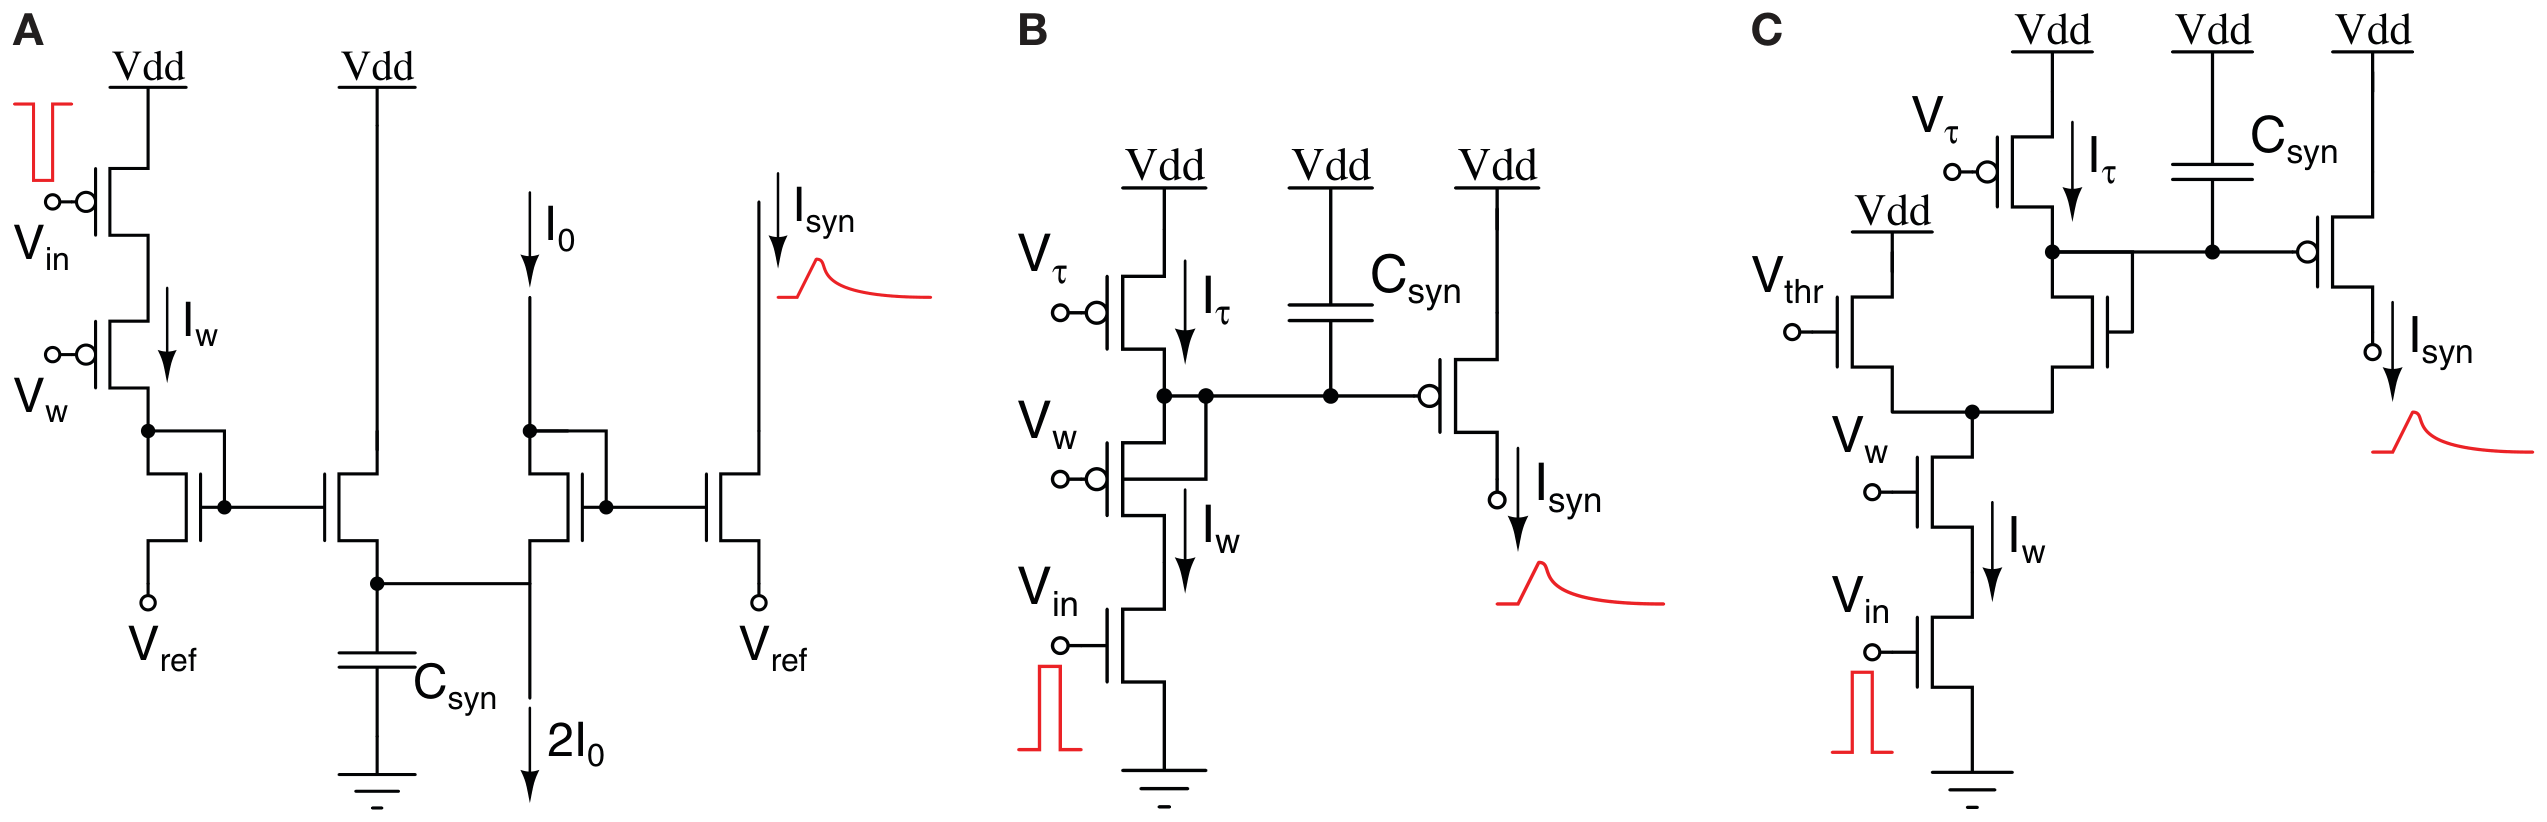
\includegraphics[width=0.98\textwidth]{indiveri_log_domain.png}
  \caption[Circuiti integratori log-domain in sottosoglia]{Circuiti integratori log-domain in sottosoglia descritti da Indiveri et al.\ (2011)~\cite{indiveri2011}: (A) circuito Tau-Cell; (B) integratore di impulsi in sottosoglia a quattro transistori; (C) Differential Pair Integrator (DPI).}
  \label{fig:log_domain}
\end{figure}

In figura~\ref{fig:log_domain} sono mostrati i tre principali circuiti integratori log-domain in sottosoglia confrontati da Indiveri et al.\ (2011)~\cite{indiveri2011}. L'idea comune a tutti e tre si vede dai segnali in rosso: in ingresso arriva uno spike di tensione $V_{\mathrm{in}}$, una tensione $V_w$ regola il peso della sinapsi generando una corrente $I_w$, il condensatore $\Csyn$ integra l'impulso e in uscita si ottiene una corrente sinaptica $\Isyn$ che cresce durante lo spike e poi scende in modo esponenziale~\cite{indiveri2011}.

Il primo circuito è la Tau-Cell (figura~\ref{fig:log_domain}A), che usa una rete di transistori in sottosoglia polarizzata tramite una tensione di riferimento $V_{\mathrm{ref}}$. Questo blocco viene usato anche dentro il soma per accumulare nel tempo gli ingressi con perdita. Lo stato della membrana è rappresentato con una corrente $\Imem$ invece che con una tensione $\Vmem$~\cite{indiveri2011}. 

Il secondo circuito è un integratore di impulsi molto semplificato (figura~\ref{fig:log_domain}B), ridotto a soli quattro transistor e alla capacità $\Csyn$~\cite{indiveri2011}. Qui la costante di tempo di scarica si regola tramite la tensione $V_\tau$ che controlla la corrente $I_\tau$~\cite{indiveri2011}. Il suo limite però è che usa un solo transistor pMOS per impostare il peso $V_w$: una volta che la costante di tempo e il peso sono stati fissati, non c'è un parametro separato per modificare l'ampiezza della corrente~\cite{indiveri2011}.

Il terzo circuito, il Differential Pair Integrator (DPI, figura~\ref{fig:log_domain}C), supera questo limite sostituendo quel singolo pMOS con una coppia differenziale collegata in retroazione negativa, a cui viene applicata una tensione di controllo aggiuntiva $V_{\mathrm{thr}}$~\cite{indiveri2011}. In questo modo l'ampiezza massima della corrente $\Isyn$ dipende da $V_w$, $V_\tau$ e anche da $V_{\mathrm{thr}}$. Questo terzo parametro permette di regolare il guadagno, cioè l'ampiezza della corrente prodotta, senza dover modificare né la costante di tempo né il peso~\cite{indiveri2011, bartels2025}. Nel paper di Bartels et al.\ (2025)~\cite{bartels2025}, in forma semplificata, la corrente d'uscita $\Isyn$ di una sinapsi DPI è espressa come:
\begin{equation}
  \tau_{\mathrm{syn}} \frac{\mathrm{d}\Isyn}{\mathrm{d}t} + \Isyn = \Iin \frac{I_w}{I_\tau},
  \qquad
  \tau_{\mathrm{syn}} = \frac{\Csyn \UT}{\kappa I_\tau},
  \label{eq:dpi_syn}
\end{equation}
dove $\Iin = I_0 \exp(\kappa V_{\mathrm{in}}/\UT)$ è la corrente dovuta allo spike in ingresso, $I_w$ è la corrente fissata dal peso sinaptico e $I_\tau$ è la corrente di polarizzazione che determina la costante di tempo $\tau_{\mathrm{syn}}$ insieme a $\Csyn$. Fino a quando dura lo spike, la corrente $\Isyn$ sale, mentre appena lo spike finisce $\Isyn$ decade esponenzialmente con costante di tempo $\tau_{\mathrm{syn}}$~\cite{indiveri2011, bartels2025}. Il DPI è il blocco scelto nei chip ROLLS, DYNAPs e DYNAP-SE2 sia per le sinapsi, sia nel soma dei neuroni AdEx-I\&F per realizzare le perdite della membrana e la corrente di adattamento~\cite{indiveri2011, qiao2015, moradi2018, bartels2025}.

Dalla relazione $\tau_{\mathrm{syn}} = \Csyn \UT / (\kappa I_\tau)$ si vede che per ottenere costanti di tempo molto lunghe mantenendo piccolo il condensatore bisogna ridurre la corrente $I_\tau$. Per salire alle centinaia di millisecondi (come nei recettori lenti NMDA in ROLLS) servono correnti nell'ordine dei picoampere o femtoampere~\cite{indiveri2011, qiao2015}. Il problema è che anche a $V_{\mathrm{GS}} = \SI{0}{\volt}$ in un transistor scorre comunque una piccola corrente di perdita. Per scendere sotto questo valore si usano gli specchi di corrente shifted-source. Tramite un traslatore di livello si alza il terminale di source dei transistori a $V_{\mathrm{nsh}} = \SI{0{,}4}{\volt}$, così da lavorare con $V_{\mathrm{GS}} < 0$ e riuscire a gestire correnti piccolissime~\cite{indiveri2011, qiao2015}. Infine per compensare il mismatch della sottosoglia, in Indiveri et al.\ (2011)~\cite{indiveri2011} descrivono il blocco Digi-MOS, una rete di transistor comandata da una parola digitale che equivale a un unico transistore di dimensione $(W/L)_{\mathrm{eff}}$ regolabile~\cite{indiveri2011}.

\subsubsection{Generazione dello spike, soglia esplicita e periodo refrattario}
Una volta che le correnti in ingresso vengono accumulate sulla membrana, serve un blocco circuitale che rileva il superamento della soglia e che genera uno spike, e che porta il neurone nella condizione di riposo~\cite{indiveri2011}.

Un esempio è il circuito Axon-Hillock di Mead, mostrato in figura~\ref{fig:spike_gen}a~\cite{indiveri2011}. La corrente d'ingresso $\Iin$ carica il condensatore $\Cmem$ facendo salire $\Vmem$ fino alla soglia di commutazione dell'amplificatore non invertente $A$. A quel punto l'uscita $V_{\mathrm{out}}$ scatta rapidamente da $0$ a $\Vdd$, attiva una retroazione positiva tramite il partitore capacitivo formato da $\Cmem$ e $C_{\mathrm{fb}}$ e accende il transistor di reset. Se la corrente di reset $I_r$ (regolata dalla tensione $V_{\mathrm{pw}}$) è maggiore di $\Iin$, il condensatore $\Cmem$ si scarica finché $\Vmem$ attraversa di nuovo la soglia dell'amplificatore. L'uscita $V_{\mathrm{out}}$ può quindi tornare a $0$ e il ciclo riparte~\cite{indiveri2011}. Il grande vantaggio di questo circuito è il basso mismatch, perché il funzionamento dipende soprattutto dal rapporto tra i due condensatori e non dai transistor~\cite{indiveri2011}.

% --- FIGURA 3.2: Axon-Hillock e van Schaik Voltage-Amplifier I&F (da Indiveri et al., 2011, Fig. 3 e 4) ---
\begin{figure}[tb]
  \centering
  \begin{subfigure}[b]{0.415\textwidth}
    \centering
    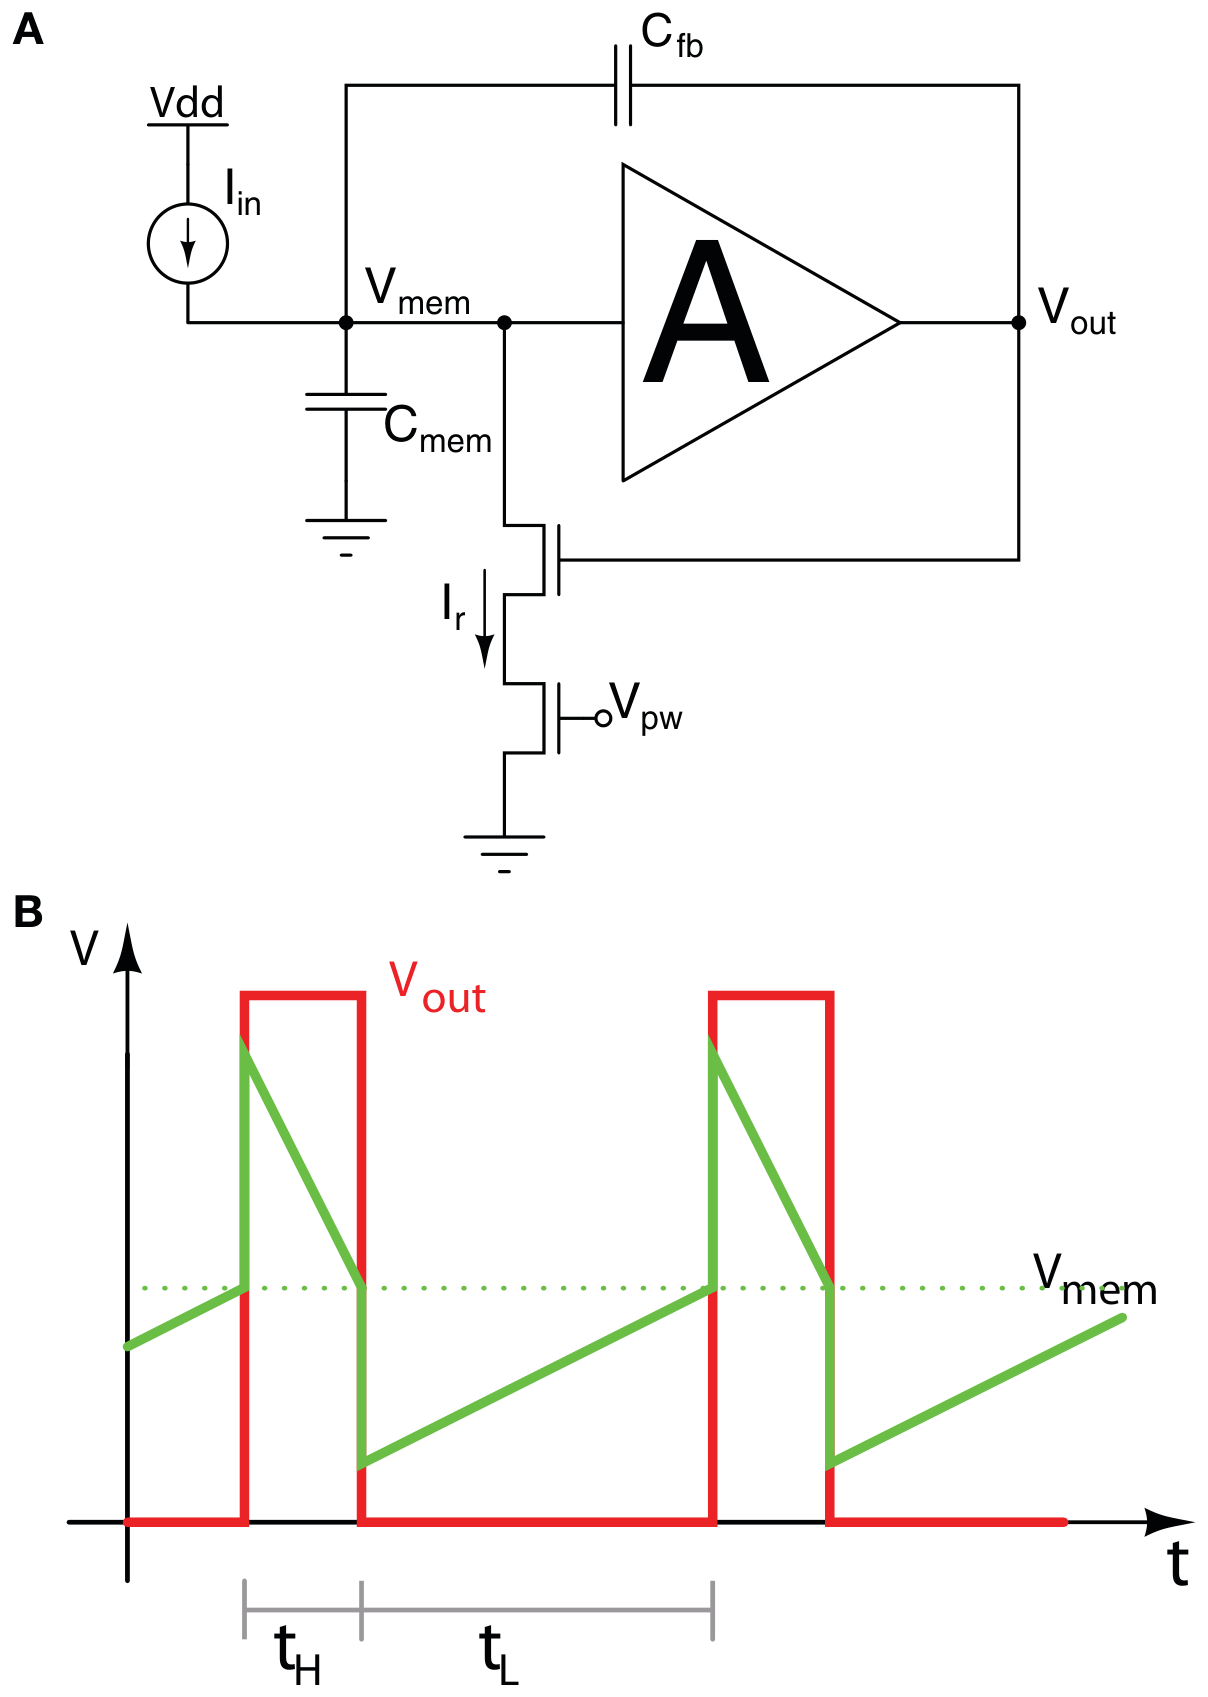
\includegraphics[width=\linewidth]{indiveri_axon_hillock.png}
    \caption{}
  \end{subfigure}
  \hfill
  \begin{subfigure}[b]{0.535\textwidth}
    \centering
    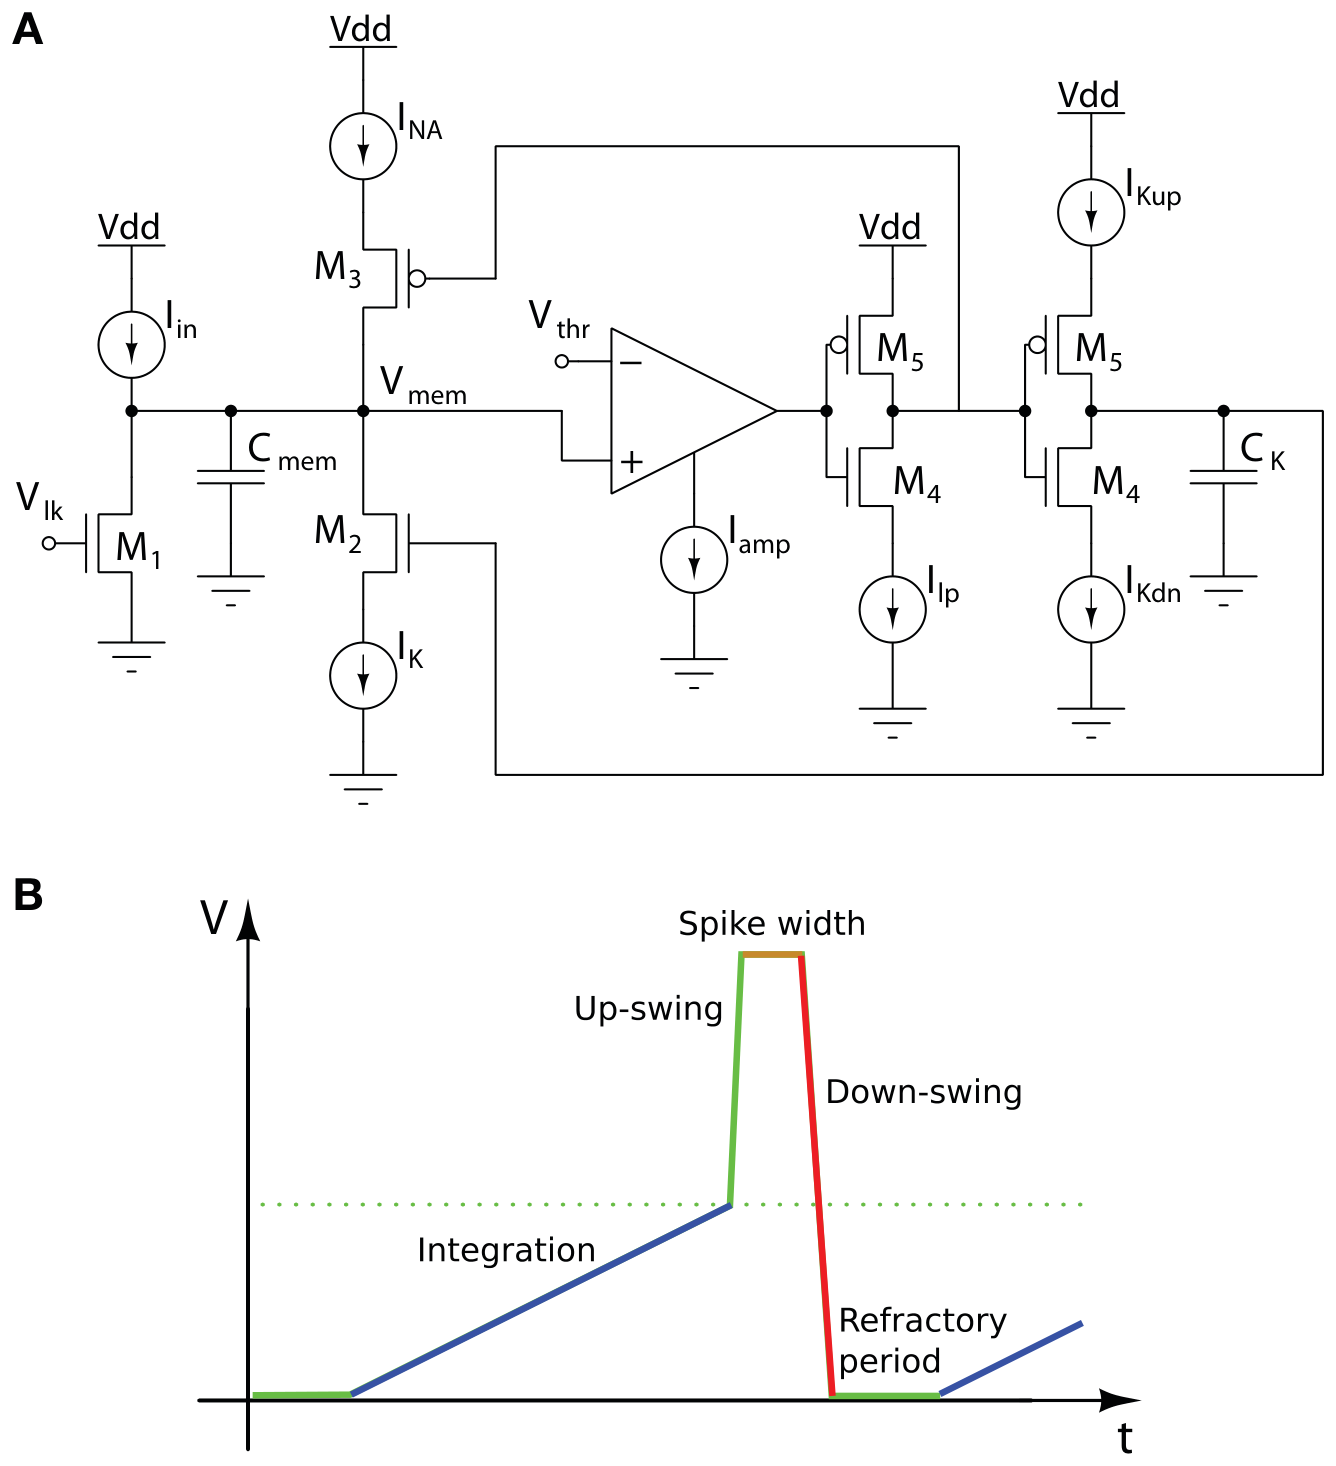
\includegraphics[width=\linewidth]{indiveri_vanschaik_ota.png}
    \caption{}
  \end{subfigure}
  \caption[]{(a) Circuito Axon-Hillock per la generazione dello spike, con schema elettrico (A) e andamento di $\Vmem$ e $V_{\mathrm{out}}$ (B); (b) Circuito di van Schaik per la generazione dello spike, con schema elettrico (A) e fasi dello spike su $\Vmem$ (B).}
  \label{fig:spike_gen}
\end{figure}

Per regolare la soglia di sparo e il periodo refrattario, van Schaik ha proposto il circuito mostrato in figura~\ref{fig:spike_gen}b~\cite{indiveri2011}. Qui il condensatore $\Cmem$ lavora assieme al transistor $M_1$ (controllato da $V_{\mathrm{lk}}$), che introduce una corrente di perdita verso massa. Se la corrente d'ingresso $\Iin$ supera questa perdita, $\Vmem$ sale e viene confrontata con una tensione di soglia  $\Vthr$ tramite un amplificatore a transconduttanza. Appena $\Vmem$ supera $\Vthr$, l'amplificatore commuta e pilota due inverter limitati in corrente (chiamati starved inverter, cioè inverter con un transistor in serie che ne fissa la corrente massima), usati per imitare l'apertura e la chiusura dei canali del sodio e del potassio~\cite{indiveri2011}. Il primo inverter accende $M_3$ lasciando scorrere la corrente $I_{\mathrm{Na}}$, che tira verso l'alto $\Vmem$. Invece il secondo inverter carica il condensatore $C_K$ con una velocità fissata dalla corrente $I_{\mathrm{Kup}}$. Quando la tensione su $C_K$ diventa abbastanza alta da accendere $M_2$, la corrente $I_K$ scarica $\Cmem$ riportando giù $\Vmem$. Quindi la corrente $I_{\mathrm{Kup}}$ regola il ritardo con cui interviene $M_2$ e fissa di conseguenza la durata dello spike. Quando $\Vmem$ scende sotto $\Vthr$, la corrente $I_{\mathrm{Na}}$ si spegne e il secondo inverter inizia a scaricare $C_K$ attraverso la corrente $I_{\mathrm{Kdn}}$. Se $I_{\mathrm{Kdn}}$ è piccola, $C_K$ si scarica lentamente mantenendo acceso $M_2$, quindi finché $I_K$ continua a scaricare la membrana, nessuna corrente d'ingresso più piccola di $I_K$ riesce a far ripartire il neurone: abbiamo ottenuto un periodo refrattario regolabile~\cite{indiveri2011}.

Però anche usando inverter limitati in corrente, quando $\Vmem$ si avvicina lentamente alla soglia resta comunque una corrente di cortocircuito tra $\Vdd$ e massa. Per ridurre questo consumo, Indiveri et al.\ (2011)~\cite{indiveri2011} propongono una soluzione, che è stata adottata nel neurone Octopus Retina. Sostanzialmente al posto della retroazione capacitiva si usa una retroazione positiva in corrente, che riutilizza la corrente di cortocircuito stessa del generatore di spike per iniettare carica aggiuntiva all'ingresso e accelerare di circa $100$ volte il superamento della soglia. La potenza di generazione dello spike è ridotta di circa $25$ volte e scende a \SI{4}{\pico\joule\per\spike} in CMOS \SI{0{,}6}{\micro\meter}~\cite{indiveri2011}.

\subsubsection{Adattamento della frequenza, neurone DPI e altri stili realizzativi}
\label{subsec:famiglie_neuroni}

I circuiti appena visti sono già dei neuroni completi molto semplici, ma non includono ancora un meccanismo per rallentare la frequenza di sparo e generare bursting. Per ottenere anche questi comportamenti, bisogna aggiungere una seconda variabile di adattamento~\cite{indiveri2011}.

Questo si può fare utilizzando i blocchi log-domain visti in precedenza. L'esempio principale di circuito CMOS completo, usato poi nei processori ROLLS, DYNAPs e DYNAP-SE2, è il neurone DPI~\cite{indiveri2011, qiao2015, moradi2018, bartels2025}. Per questo circuito valgono le seguenti equazioni~\cite{indiveri2011}:
\begin{equation}
  \tau \frac{\mathrm{d}\Imem}{\mathrm{d}t} = -\Imem\!\left(1 + \frac{I_g}{I_\tau}\right) + I_{\mathrm{mem}\infty} + f(\Imem),
  \qquad
  \tau_g \frac{\mathrm{d}I_g}{\mathrm{d}t} = -I_g + I_{g\max}\,r(t),
  \label{eq:dpi_adex}
\end{equation}
dove $\tau = \Cmem\UT/(\kappa I_\tau)$ è la costante di tempo di membrana, $I_{\mathrm{mem}\infty}$ dipende dalla corrente d'ingresso $\Iin$, $f(\Imem)$ è un termine esponenziale e $r(t)$ vale $1$ durante lo spike e $0$ altrimenti~\cite{indiveri2011}.

Se la priorità è invece ridurre il mismatch, in Indiveri et al.\ (2011)~\cite{indiveri2011} vengono mostrate alcune soluzioni alternative alla sottosoglia. Lavorando in forte inversione ma senza usare condensatori esterni, si passa a circuiti con costanti di tempo molto più veloci di quelle biologiche ($10^3\text{--}10^5$ volte, come nel neurone quadratico di Izhikevich di Wijekoon e Dudek in CMOS \SI{0{,}35}{\micro\meter}, circa $10^4$ volte più veloce)~\cite{indiveri2011}. Se invece si vuole restare nell'ordine dei tempi biologici, il neurone di Mihalas--Niebur a capacità commutate usa interruttori comandati da più fasi di clock~\cite{indiveri2011}. Per compensare il mismatch si possono anche usare i blocchi Digi-MOS già visti, mentre per eliminarlo del tutto si può ricorrere a neuroni LIF interamente digitali, basati su sommatori e accumulatori~\cite{indiveri2011}.

\subsection{Analisi approfondita dei processori CMOS della bibliografia}
\label{subsec:processori_cmos}

\subsubsection{ROLLS (Qiao et al., 2015): processore mixed-signal con apprendimento on-line}
\label{subsec:rolls_cmos}

Il processore ROLLS (Reconfigurable On-Line Learning Spiking neuromorphic processor) mostrato nel paper di Qiao et al.~\cite{qiao2015}, è un chip mixed-signal progettato per realizzare reti neurali spiking riconfigurabili con apprendimento direttamente sul chip e in tempo reale. È fabbricato in CMOS \SI{180}{\nano\meter}, occupa un'area di \SI{51{,}4}{\milli\meter\squared} con circa 12,2 milioni di transistor e consuma in media circa \SI{4}{\milli\watt}~\cite{qiao2015}.

È fatto da 256 neuroni analogici AdEx-I\&F e da 128k sinapsi analogiche, divise in due matrici $256\times 256$: 64k sinapsi con plasticità a lungo termine (LTP) per l'apprendimento sul chip e 64k sinapsi programmabili con plasticità a breve termine (STP)~\cite{qiao2015}. Un blocco di demultiplexing permette inoltre di assegnare più righe di sinapsi a uno stesso neurone, sacrificando i neuroni non utilizzati~\cite{qiao2015}.

% --- FIGURA 3.3: Schema CMOS del neurone AdEx-I&F di ROLLS (da Qiao et al., 2015, Fig. 3) ---
\begin{figure}[tb]
  \centering
  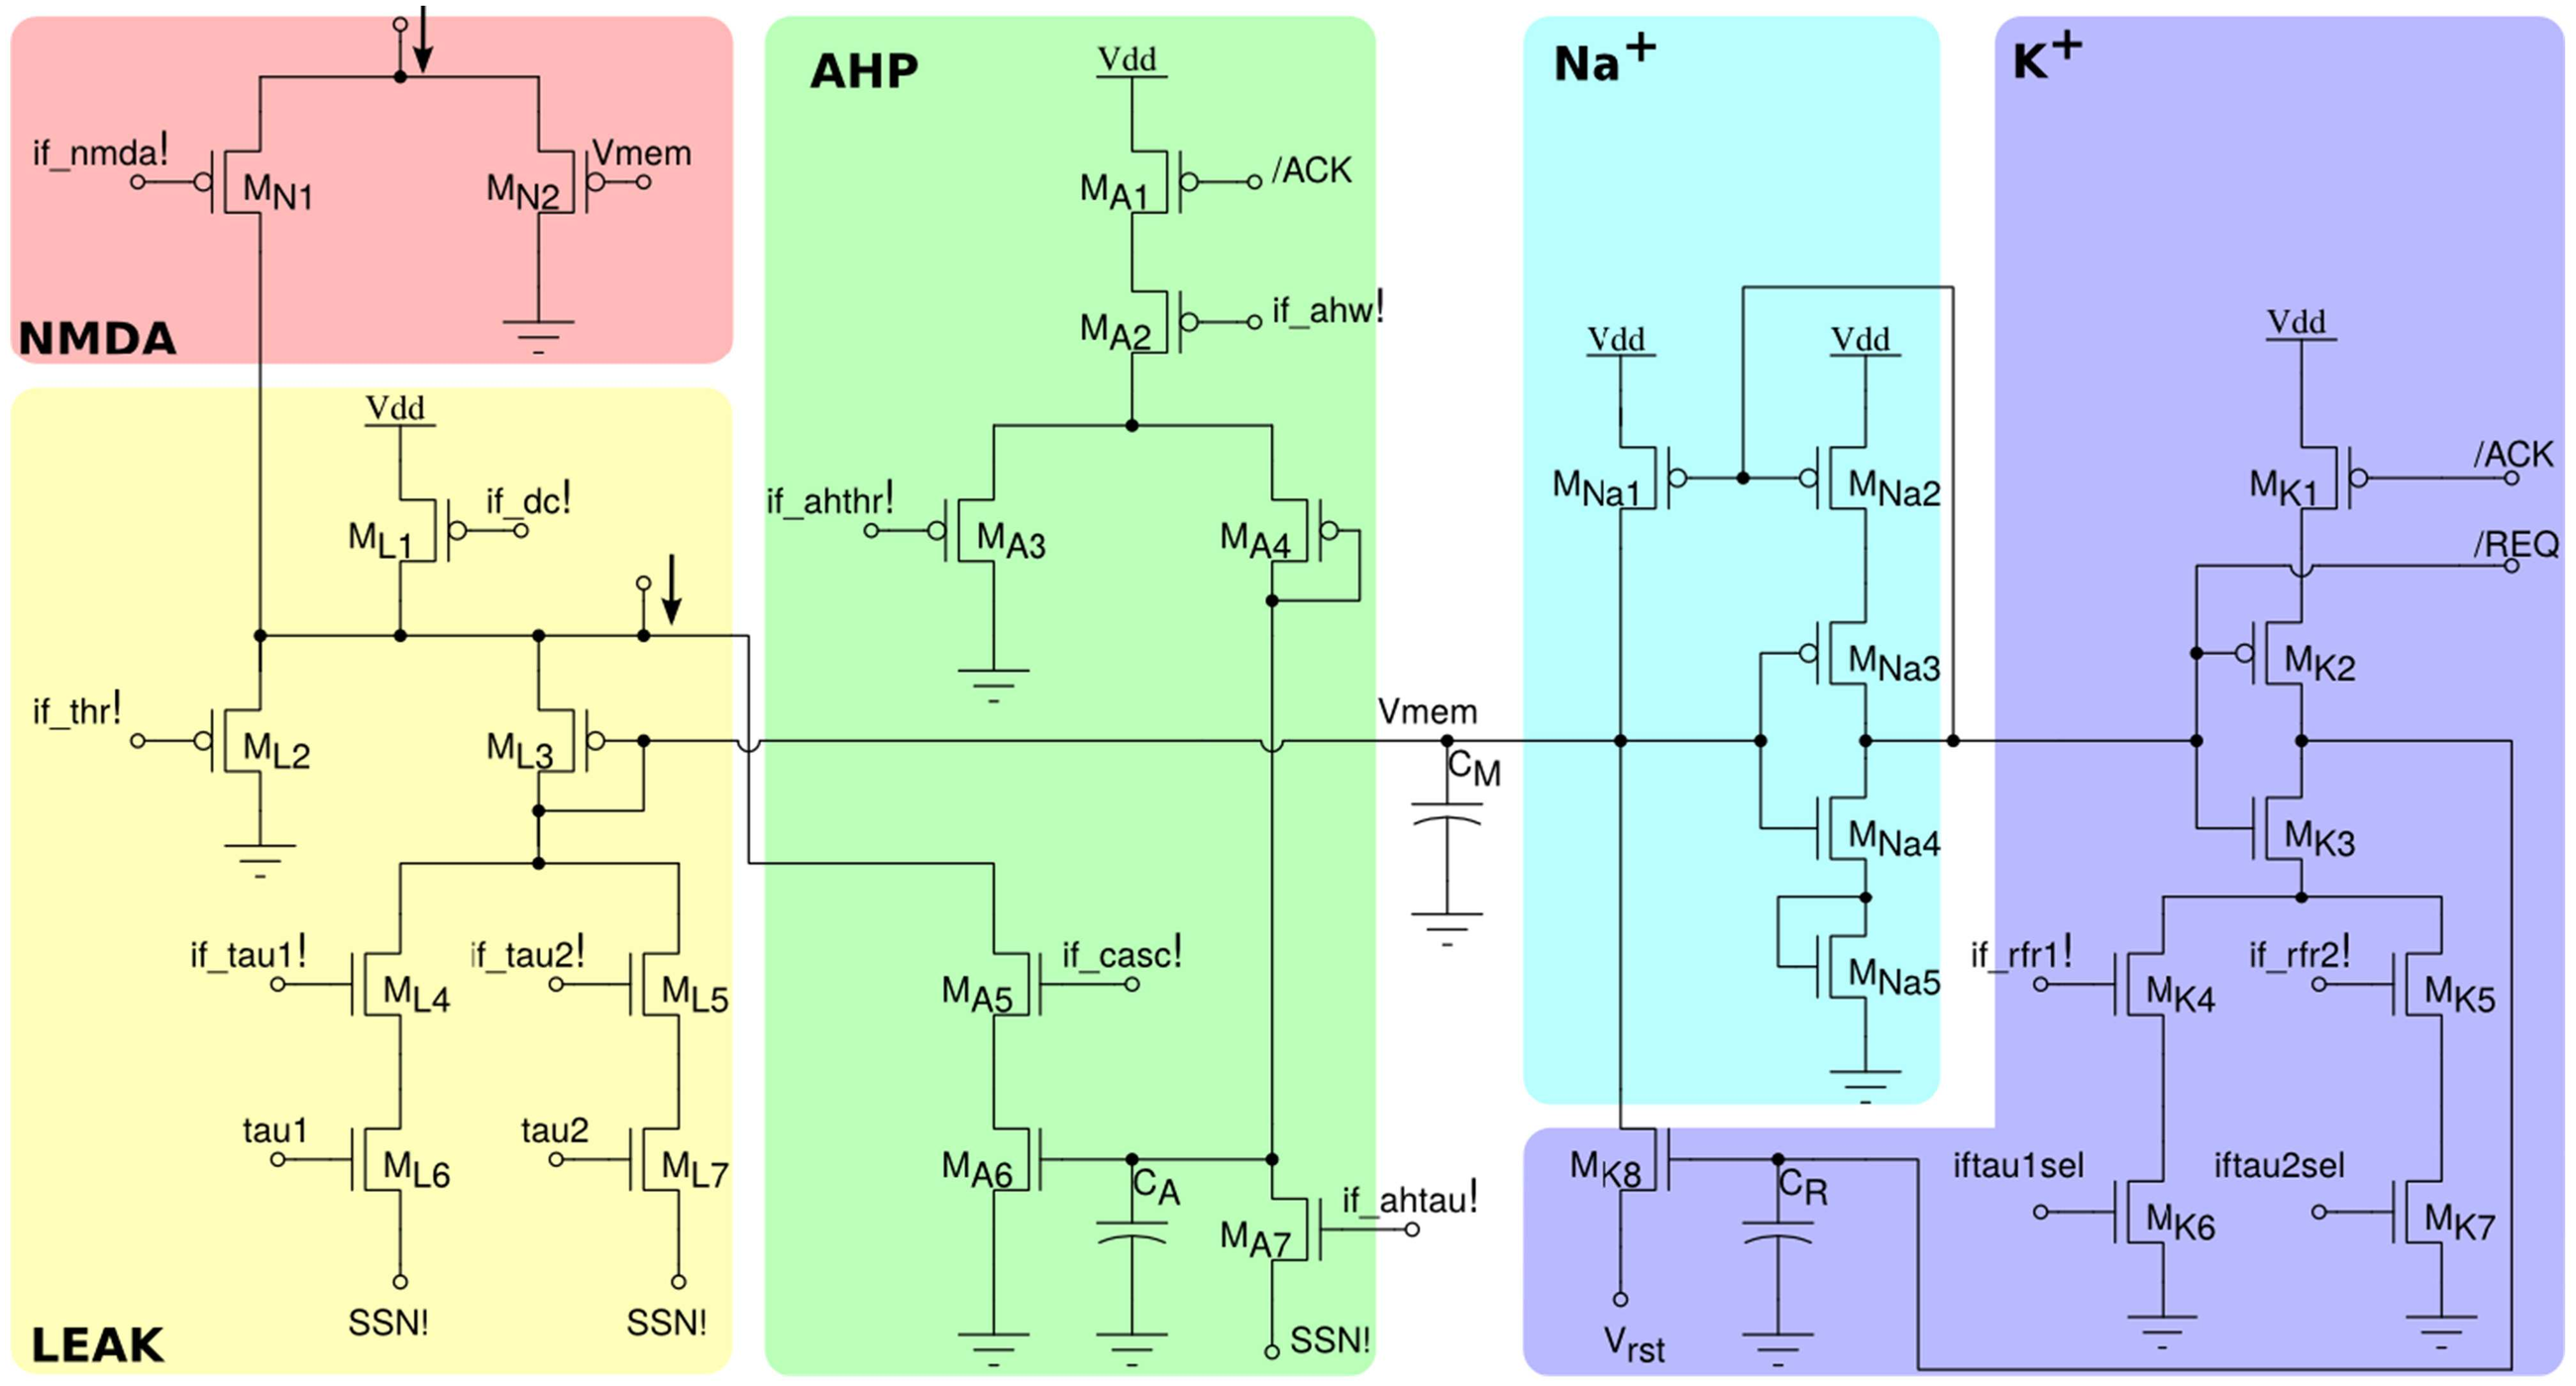
\includegraphics[width=\textwidth]{rolls_neuron_schematic.png}
  \caption[Schema CMOS del neurone AdEx-I\&F di ROLLS]{Schema a livello di transistor del neurone AdEx-I\&F del processore ROLLS~\cite{qiao2015}, suddiviso nei cinque blocchi funzionali (NMDA, LEAK, AHP, $\mathrm{Na}^+$ e $\mathrm{K}^+$).}
  \label{fig:rolls_neuron_schematic}
\end{figure}

In figura~\ref{fig:rolls_neuron_schematic} è riportato lo schema a livello di transistor del neurone di ROLLS~\cite{qiao2015}. Il circuito ha 13 bias regolabili (quelli indicati con il punto esclamativo nello schema) ed è organizzato in cinque blocchi. Il blocco NMDA ($M_{N1}, M_{N2}$) regola le correnti sinaptiche in funzione del potenziale di membrana $\Vmem$. Il blocco LEAK ($M_{L1}\text{--}M_{L7}$) è il circuito DPI d'ingresso che modella la perdita della membrana sulla capacità $C_M$. Sottolineo che usa la polarizzazione shifted-source (\texttt{SSN!}) vista in precedenza, per ottenere costanti di tempo biologiche. Il blocco AHP ($M_{A1}\text{--}M_{A7}$) integra gli spike emessi dal neurone sulla capacità $C_A$ (a ogni conferma \texttt{/ACK} ricevuta dal bus AER) e produce una corrente che frena il neurone, ottenendo adattamento della frequenza e bursting. Il blocco $\mathrm{Na}^+$ ($M_{\mathrm{Na1}}\text{--}M_{\mathrm{Na5}}$) applica la retroazione positiva in corrente al superamento della soglia per far salire rapidamente lo spike, imitando i canali del sodio. Infine il blocco $\mathrm{K}^+$ ($M_{K1}\text{--}M_{K8}$) segnala lo spike al bus AER tramite il segnale di richiesta \texttt{/REQ} (per trasmettere l'indirizzo del neurone), imposta il periodo refrattario tramite il condensatore $C_R$ e riporta $\Vmem$ al potenziale di reset regolabile $V_{\mathrm{rst}}$~\cite{qiao2015}. Inoltre, potendo selezionare digitalmente per ogni neurone tra due costanti di tempo di perdita nel blocco LEAK e due periodi refrattari nel blocco $\mathrm{K}^+$, si possono configurare fino a quattro popolazioni diverse di neuroni sullo stesso chip~\cite{qiao2015}. I comportamenti misurati sul silicio (reset regolabile, periodo refrattario, adattamento della frequenza e bursting) sono mostrati in figura~\ref{fig:rolls_silicio}c~\cite{qiao2015}.

Un aspetto importante del progetto di ROLLS è la riduzione del mismatch analogico. In sottosoglia le variazioni tra transistor possono rendere i neuroni molto diversi tra loro; per limitare questo effetto, gli autori hanno aumentato in modo mirato le dimensioni dei transistor più critici del soma, cioè quelli che fissano la costante di tempo di perdita ($M_{L4}$ e $M_{L5}$, con $W/L = \SI{2}{\micro\meter}/\SI{4}{\micro\meter}$) e la soglia di sparo ($M_{\mathrm{Na3}}$ da $\SI{4}{\micro\meter}/\SI{0{,}4}{\micro\meter}$ e $M_{\mathrm{Na4}}$ da $\SI{1}{\micro\meter}/\SI{4}{\micro\meter}$). Come si vede dalla curva frequenza-corrente in figura~\ref{fig:rolls_silicio}b, il mismatch medio su tutti i 256 neuroni scende così al 9,4\%, un valore molto contenuto per circuiti analogici in sottosoglia~\cite{qiao2015}.

\begin{figure}[tb]
  \centering
  \begin{subfigure}[b]{0.48\textwidth}
    \centering
    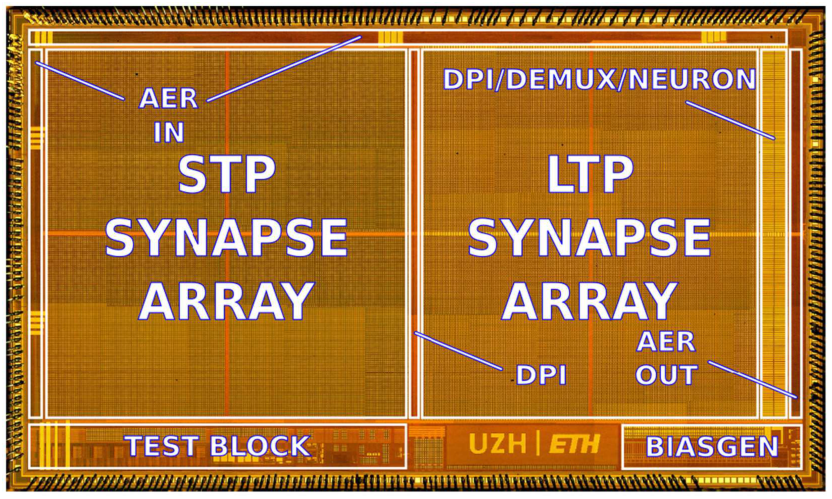
\includegraphics[width=\linewidth]{rolls_die.png}
    \caption{}
  \end{subfigure}
  \hfill
  \begin{subfigure}[b]{0.48\textwidth}
    \centering
    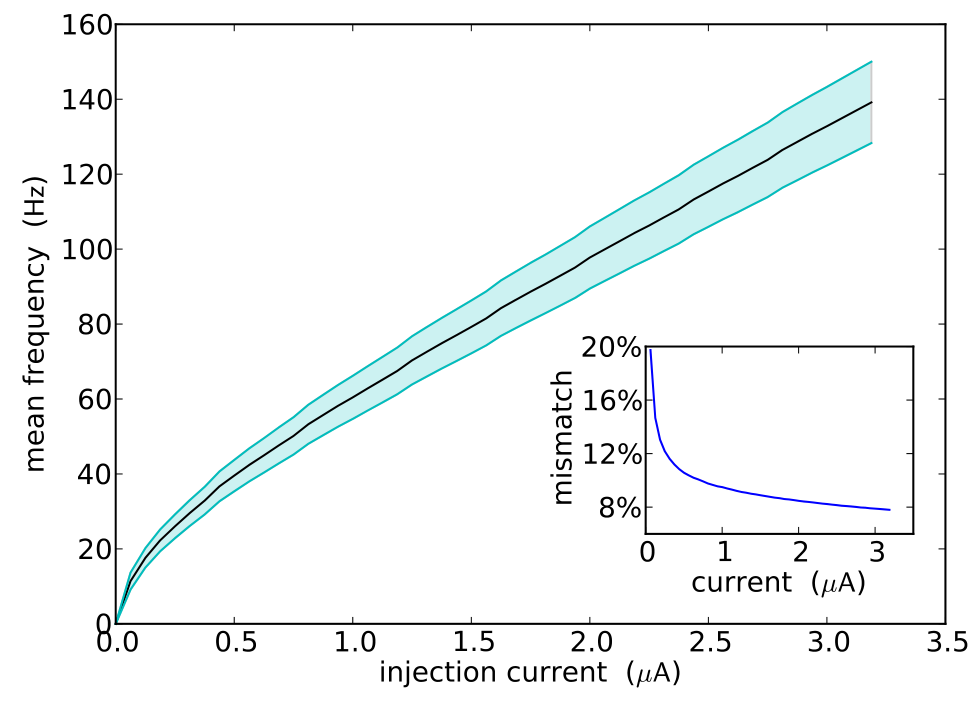
\includegraphics[width=\linewidth]{rolls_fi_mismatch.png}
    \caption{}
  \end{subfigure}
  \vspace{0.3cm}
  \begin{subfigure}[b]{0.92\textwidth}
    \centering
    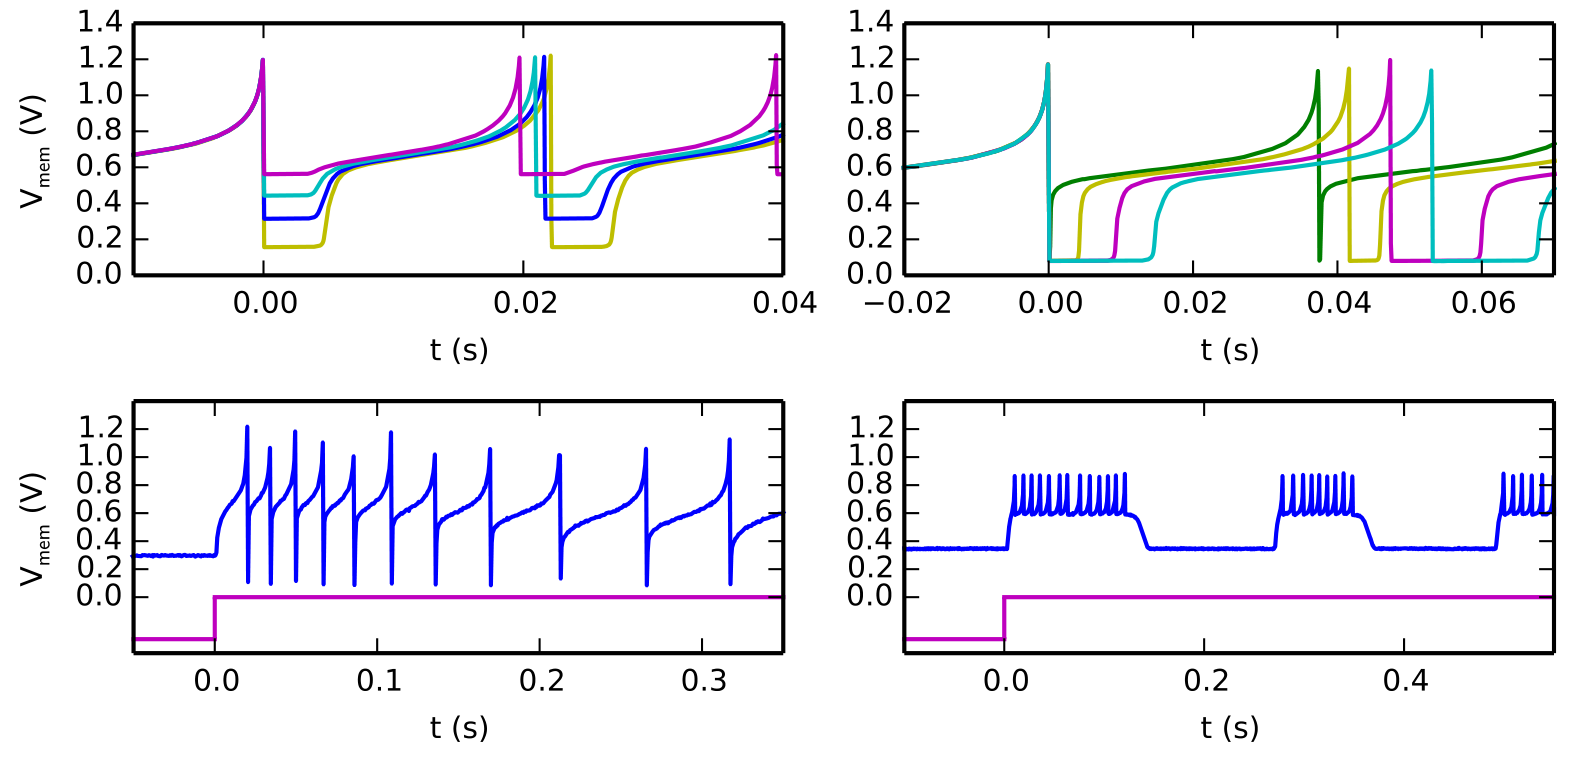
\includegraphics[width=\linewidth]{rolls_behaviors.png}
    \caption{}
  \end{subfigure}
  \caption[Caratterizzazione sperimentale del processore ROLLS]{Caratterizzazione sperimentale di ROLLS~\cite{qiao2015}: (a) microfotografia del die (\SI{51{,}4}{\milli\meter\squared} in CMOS \SI{180}{\nano\meter}); (b) curva frequenza-corrente media e deviazione standard dei 256 neuroni (mismatch medio 9,4\%); (c) andamenti misurati di $\Vmem$ per reset regolabile, periodo refrattario, adattamento della frequenza e bursting.}
  \label{fig:rolls_silicio}
\end{figure}

Per quanto riguarda le sinapsi, ROLLS adotta due soluzioni principali. La prima serve a risparmiare area: assumendo che le sinapsi di una stessa riga condividano le stesse costanti di tempo, le loro correnti d'uscita vengono sommate sfruttando la legge di Kirchhoff in un unico circuito DPI condiviso per riga (un DPI lento di tipo NMDA nella matrice LTP con costanti di tempo di centinaia di millisecondi, e due DPI più veloci di tipo AMPA e GABA nella matrice STP con costanti di tempo di decine di millisecondi)~\cite{qiao2015}. La seconda riguarda l'apprendimento e la conservazione dei pesi nel tempo. Nella matrice LTP i pesi analogici vengono aggiornati secondo la regola bistabile con stop-learning di Brader et al.\ (2007): all'arrivo di uno spike pre-sinaptico, la tensione interna $V_w$ che rappresenta il peso viene aumentata o diminuita in base al potenziale di membrana $\Vmem$ e all'attività recente del neurone post-sinaptico (modellata come una concentrazione di calcio misurata da un circuito DPI dedicato e confrontata con tre soglie per decidere se aggiornare o fermare l'apprendimento); in parallelo, un amplificatore a retroazione positiva spinge lentamente $V_w$ verso uno dei due stati stabili (alto o basso), evitando che il peso analogico vada alla deriva sul lungo periodo~\cite{qiao2015}. Nella matrice STP, invece, ogni sinapsi ha un peso digitale programmabile a 2 bit (quattro livelli), un bit per impostarla come eccitatoria o inibitoria e, in modalità eccitatoria, un circuito analogico di depressione a breve termine (STD) che riduce temporaneamente l'ampiezza della corrente durante raffiche di spike ravvicinati~\cite{qiao2015}.

Nonostante la condivisione dei circuiti DPI per riga, la ripartizione dell'area del chip (visibile anche in figura~\ref{fig:rolls_silicio}a) mette in evidenza un risultato molto significativo: i 256 neuroni ($55{,}69 \times \SI{16{,}48}{\micro\meter\squared}$ ciascuno, pari a \SI{0{,}235}{\milli\meter\squared} in totale) occupano solo lo 0,47\% dell'intera superficie del die, mentre le 128k sinapsi LTP (31,41\%) e STP (33,32\%) assorbono insieme il 64,73\% dell'area (\SI{33{,}28}{\milli\meter\squared}), con il resto occupato da generatore di bias, interfacce AER, logica di supporto e pad~\cite{qiao2015}.

\subsubsection{NET-TEN (Ronchini et al., 2023): rete analogica ultra-low-power a 250 mV}
\label{subsec:netten_cmos}

A differenza di un processore general-purpose riconfigurabile come ROLLS, \textbf{NET-TEN}~\cite{ronchini2023} dimostra cosa accade quando l'intera architettura CMOS viene progettata su misura per un'applicazione impiantabile, eliminando routing digitale, memorie SRAM/CAM e BiasGen integrati. Fabbricato anch'esso in CMOS \SI{180}{\nano\meter} ma alimentato a soli \textbf{$\Vdd = \SI{250}{\milli\volt}$}, il chip occupa \SI{1{,}08}{\milli\meter\squared} e integra 30 neuroni Izhikevich sottosoglia organizzati in 3 strati \emph{feed-forward} sparsi (10--10--10, con fan-in e fan-out pari a 2 tra primo e secondo strato e connessioni 1-a-1 tra strato nascosto e uscita) più 30 sinapsi EPSC+STDP (Figura~\ref{fig:netten_circuits})~\cite{ronchini2023}.

% --- FIGURA 3.5: Topologia, Neurone Izhikevich, EPSC e STDP di NET-TEN (da Ronchini et al., 2023, Fig. 3) ---
\begin{figure}[tb]
  \centering
  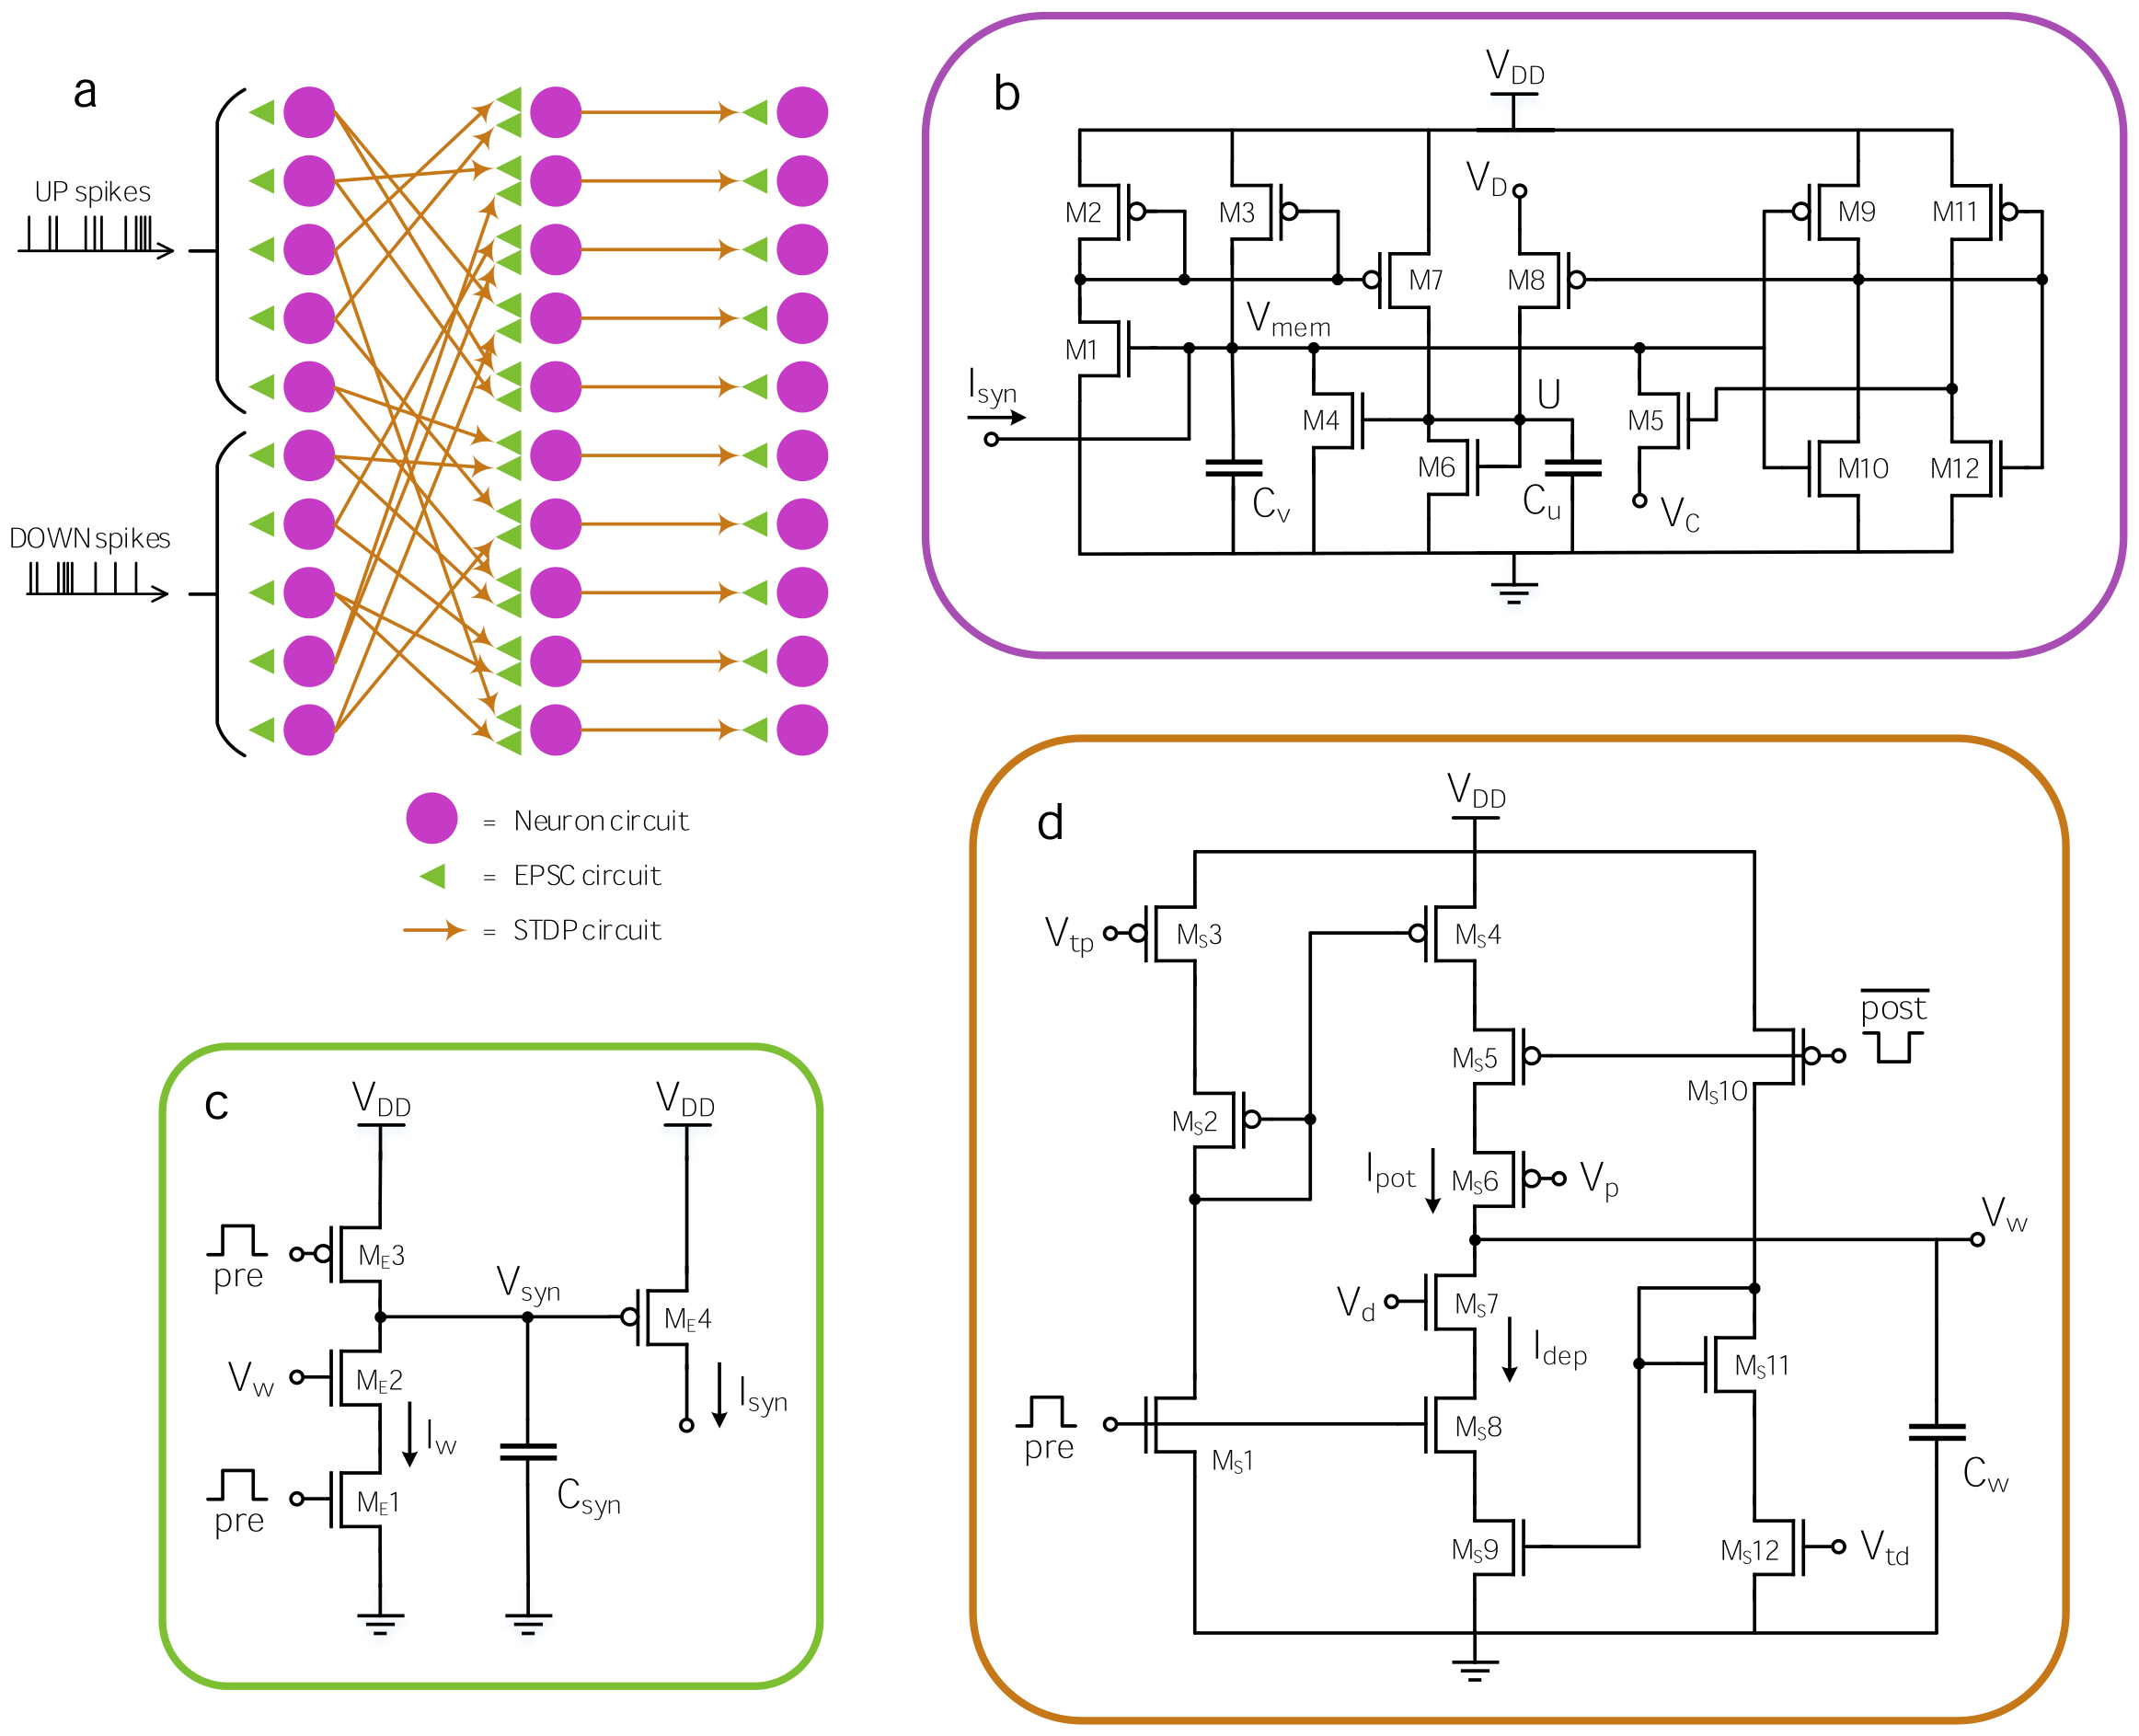
\includegraphics[width=0.90\textwidth]{netten_circuits.png}
  \caption[Topologia e schemi CMOS sottosoglia di NET-TEN]{Architettura e schemi CMOS sottosoglia di NET-TEN~\cite{ronchini2023} ($\Vdd = \SI{250}{\milli\volt}$): (a) topologia \emph{feed-forward} sparsa a 3 strati da 10 neuroni ciascuno; (b) neurone Izhikevich \emph{voltage-mode} ($M_1\text{--}M_{12}$, $C_v = \SI{76{,}86}{\femto\farad}$, $C_u = \SI{614{,}88}{\femto\farad}$, area \SI{1476{,}84}{\micro\meter\squared}); (c) generatore EPSC ($M_{E1}\text{--}M_{E4}$, picco \SI{486{,}39}{\pico\ampere}, $\tau = \SI{212{,}83}{\micro\second}$, area \SI{462{,}09}{\micro\meter\squared}); (d) circuito STDP sottosoglia ($M_{S1}\text{--}M_{S12}$, $C_w = \SI{206{,}30}{\femto\farad}$, area \SI{1054{,}75}{\micro\meter\squared}). Riprodotto da Ronchini et al.\ (2023)~\cite{ronchini2023}, licenza CC BY 4.0.}
  \label{fig:netten_circuits}
\end{figure}

Nel neurone di NET-TEN (Figura~\ref{fig:netten_circuits}b, area \SI{1476{,}84}{\micro\meter\squared}), le due variabili di stato del modello di Izhikevich ($\Vmem$ e $U$) risiedono sui condensatori integrati $C_v = \SI{76{,}86}{\femto\farad}$ e $C_u = \SI{614{,}88}{\femto\farad}$ (ottimizzati mediante analisi Monte Carlo per attenuare le variazioni di processo). Lo specchio $M_1\text{--}M_3$ applica un feedback positivo su $\Vmem$, bilanciato dalla corrente di leak $I_{M4}$ controllata da $U$; lo specchio $M_1, M_2, M_7$ accoppia $\Vmem$ a $U$, mentre $M_6$ fornisce il decadimento negativo su $C_u$. Due inverter in cascata ($M_9\text{--}M_{12}$) fungono da comparatore a soglia fissa generando sia l'impulso negativo di reset di $U$ (tramite $M_8$ e $V_D$) sia quello positivo di reset di $\Vmem$ (tramite $M_5$ e $V_C$). Il circuito EPSC ($M_{E1}\text{--}M_{E4}$, area \SI{462{,}09}{\micro\meter\squared}, Figura~\ref{fig:netten_circuits}c) precarica $C_{\mathrm{syn}}$ a $\Vdd$ tramite $M_{E3}$ e lo scarica all'arrivo dello spike \texttt{pre} con una corrente proporzionale al peso $V_w$, producendo su $M_{E4}$ (in sottosoglia) una corrente post-sinaptica esponenziale con picco di \SI{486{,}39}{\pico\ampere} e costante di tempo $\tau = \SI{212{,}83}{\micro\second}$ (a $V_w = \SI{200}{\milli\volt}$). Infine, il circuito STDP sottosoglia (derivato da Indiveri, area \SI{1054{,}75}{\micro\meter\squared}, Figura~\ref{fig:netten_circuits}d) memorizza il peso su $C_w = \SI{206{,}30}{\femto\farad}$, garantendo un'evoluzione adattativa su scale di decine di millisecondi~\cite{ronchini2023}.

NET-TEN mette in luce con grande chiarezza i due compromessi fisici del design interamente sottosoglia a \SI{250}{\milli\volt}:
\begin{itemize}
  \item \textbf{Variabilità (\emph{mismatch}) bifronte:} con bias globali identici, il \emph{mismatch} crea una naturale diversità funzionale fra neuroni (utile come espansione in caratteristiche casuali), ma oltre una certa soglia rende alcuni neuroni silenti o sempre attivi — motivo per cui solo 4 canali su 10 risultano utili e non sono identificabili a priori~\cite{ronchini2023}.
  \item \textbf{Ridotta capacità di pilotaggio (\emph{drivability}):} le correnti sub-nanoampere limitano il \emph{fan-out} senza ingrandire i transistori, imponendo la connettività sparsa (fan-out 2) e rendendo necessari buffer operazionali esterni (MAX44280, capacità d'ingresso \SI{0{,}4}{\pico\farad}) per osservare le uscite su PCB~\cite{ronchini2023}.
\end{itemize}

\subsubsection{DYNAPs (Moradi et al., 2018): scalabilità multi-core, memorie eterogenee e routing asincrono}
\label{subsec:dynaps_cmos}

Quando si passa da piccole reti dedicate (30 neuroni in NET-TEN) o da un singolo array (256 neuroni in ROLLS) a sistemi neuromorfici scalabili con migliaia o milioni di neuroni ed elevato \emph{fan-out} ($F \sim 10^3\text{--}10^4$), il vero collo di bottiglia non è più il circuito del singolo neurone, bensì la \textbf{memoria necessaria per memorizzare la connettività e l'energia per instradare gli spike}~\cite{moradi2018}.

In uno schema di routing convenzionale punto-punto per $N$ neuroni con fan-out $F$, ciascun neurone deve memorizzare $F \log_2(N)$ bit di indirizzi (es.\ \SI{160}{\kilo\bit\per\text{neurone}} per $N = 2^{20} \approx 10^6$ e $F \approx 10^4$). Per abbattere tale costo senza sacrificare la programmabilità né ricorrere a DRAM esterne, Moradi et al.\ (2018)~\cite{moradi2018} introducono nei processori \textbf{DYNAPs} (\emph{Dynamic Neuromorphic Asynchronous Processors}) uno \textbf{schema di routing a due stadi basato su tag condivisi}, ispirato alla connettività a cluster della corteccia cerebrale:
\begin{enumerate}
  \item i neuroni sono raggruppati in $N/C$ core (cluster) di dimensione $C$;
  \item nel \textbf{primo stadio} (routing sorgente punto-punto), il router locale \textbf{R1} legge una SRAM di sorgente e invia un \emph{tag} di $\log_2(K)$ bit a $F/M$ nodi intermedi (core di destinazione);
  \item nel \textbf{secondo stadio} (\emph{broadcast} locale), il tag viene diffuso a tutti i $C$ neuroni del core di destinazione, ciascuno dotato di una memoria associativa asincrona \textbf{CAM} (\emph{Content-Addressable Memory}) che accetta lo spike solo se il tag coincide con una delle sue sinapsi sottoscritte ($M$ neuroni sottoscritti per tag; Figura~\ref{fig:dynaps_routing}b).
\end{enumerate}

Minimizzando la somma di memoria sorgente $\mathrm{MEM}_S$ e memoria destinazione $\mathrm{MEM}_T$ rispetto al parametro di compromesso $M$ (con $\alpha = K/C = 1$), Moradi et al.\ dimostrano che la memoria per neurone si riduce a~\cite{moradi2018}:
\begin{equation}
  \mathrm{MEM} = \frac{F}{M}\log_2\!\left(\frac{KN}{C}\right) + \frac{KM}{C}\log_2(K)
  \;\xrightarrow[\alpha=1]{M = M^*}\;
  \mathrm{MEM}_{\min} = 2\sqrt{F \log_2(C)\log_2(N)}\;\;\text{bit/neurone}.
  \label{eq:dynaps_mem}
\end{equation}
Per una rete da un milione di neuroni ($N=2^{20}$, $F=2^{13}$, $C=256$), ciò abbatte la memoria da \textbf{160k bit/neurone a meno di 1,2k bit/neurone} (oltre $130\times$ di riduzione), assicurando inoltre uno scaling lineare anziché quadratico rispetto a IBM TrueNorth nell'implementazione di CNN~\cite{moradi2018}.

% --- FIGURA 3.6: Architettura di routing R1-R2-R3 e nodo eterogeneo DYNAPs (da Moradi et al., 2018, Fig. 2 e 9) ---
\begin{figure}[tbp]
  \centering
  \begin{subfigure}[b]{0.48\textwidth}
    \centering
    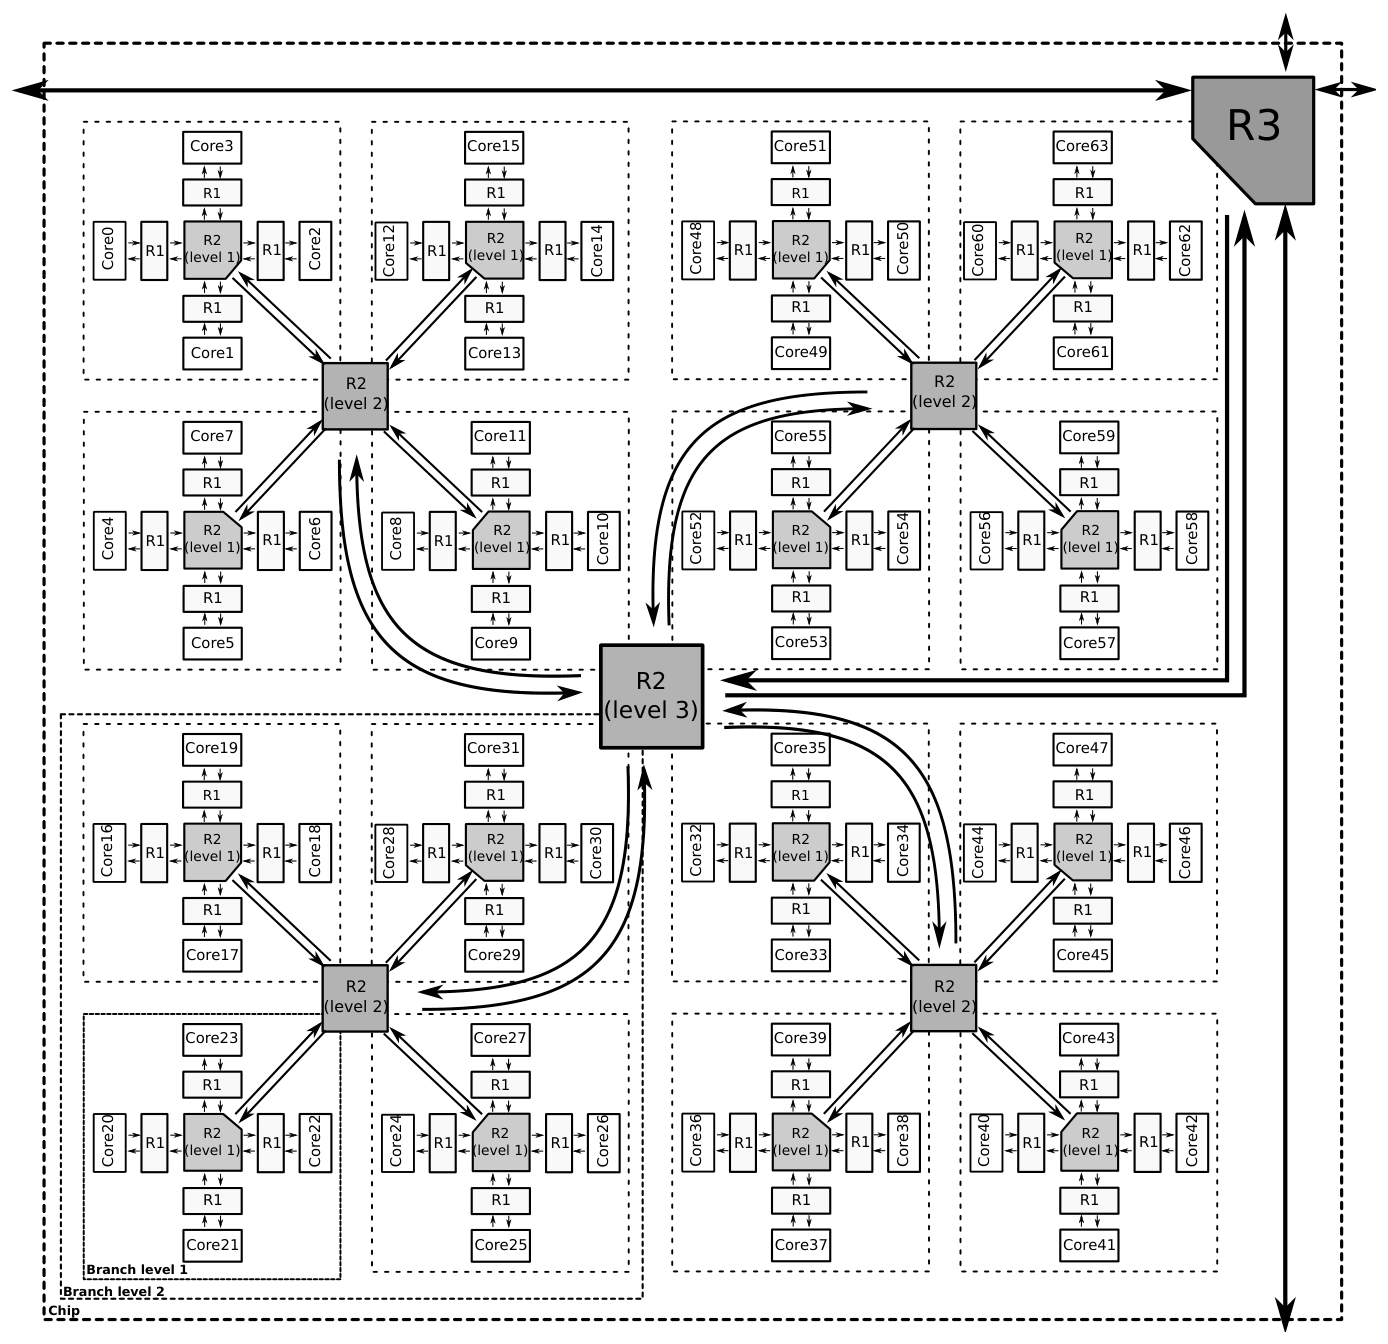
\includegraphics[width=\linewidth]{dynaps_routing_tree.png}
    \caption{Rete di routing gerarchica ad albero (R1, R2) e mesh 2D (R3).}
  \end{subfigure}

  \vspace{0.35cm}
  \begin{subfigure}[b]{0.76\textwidth}
    \centering
    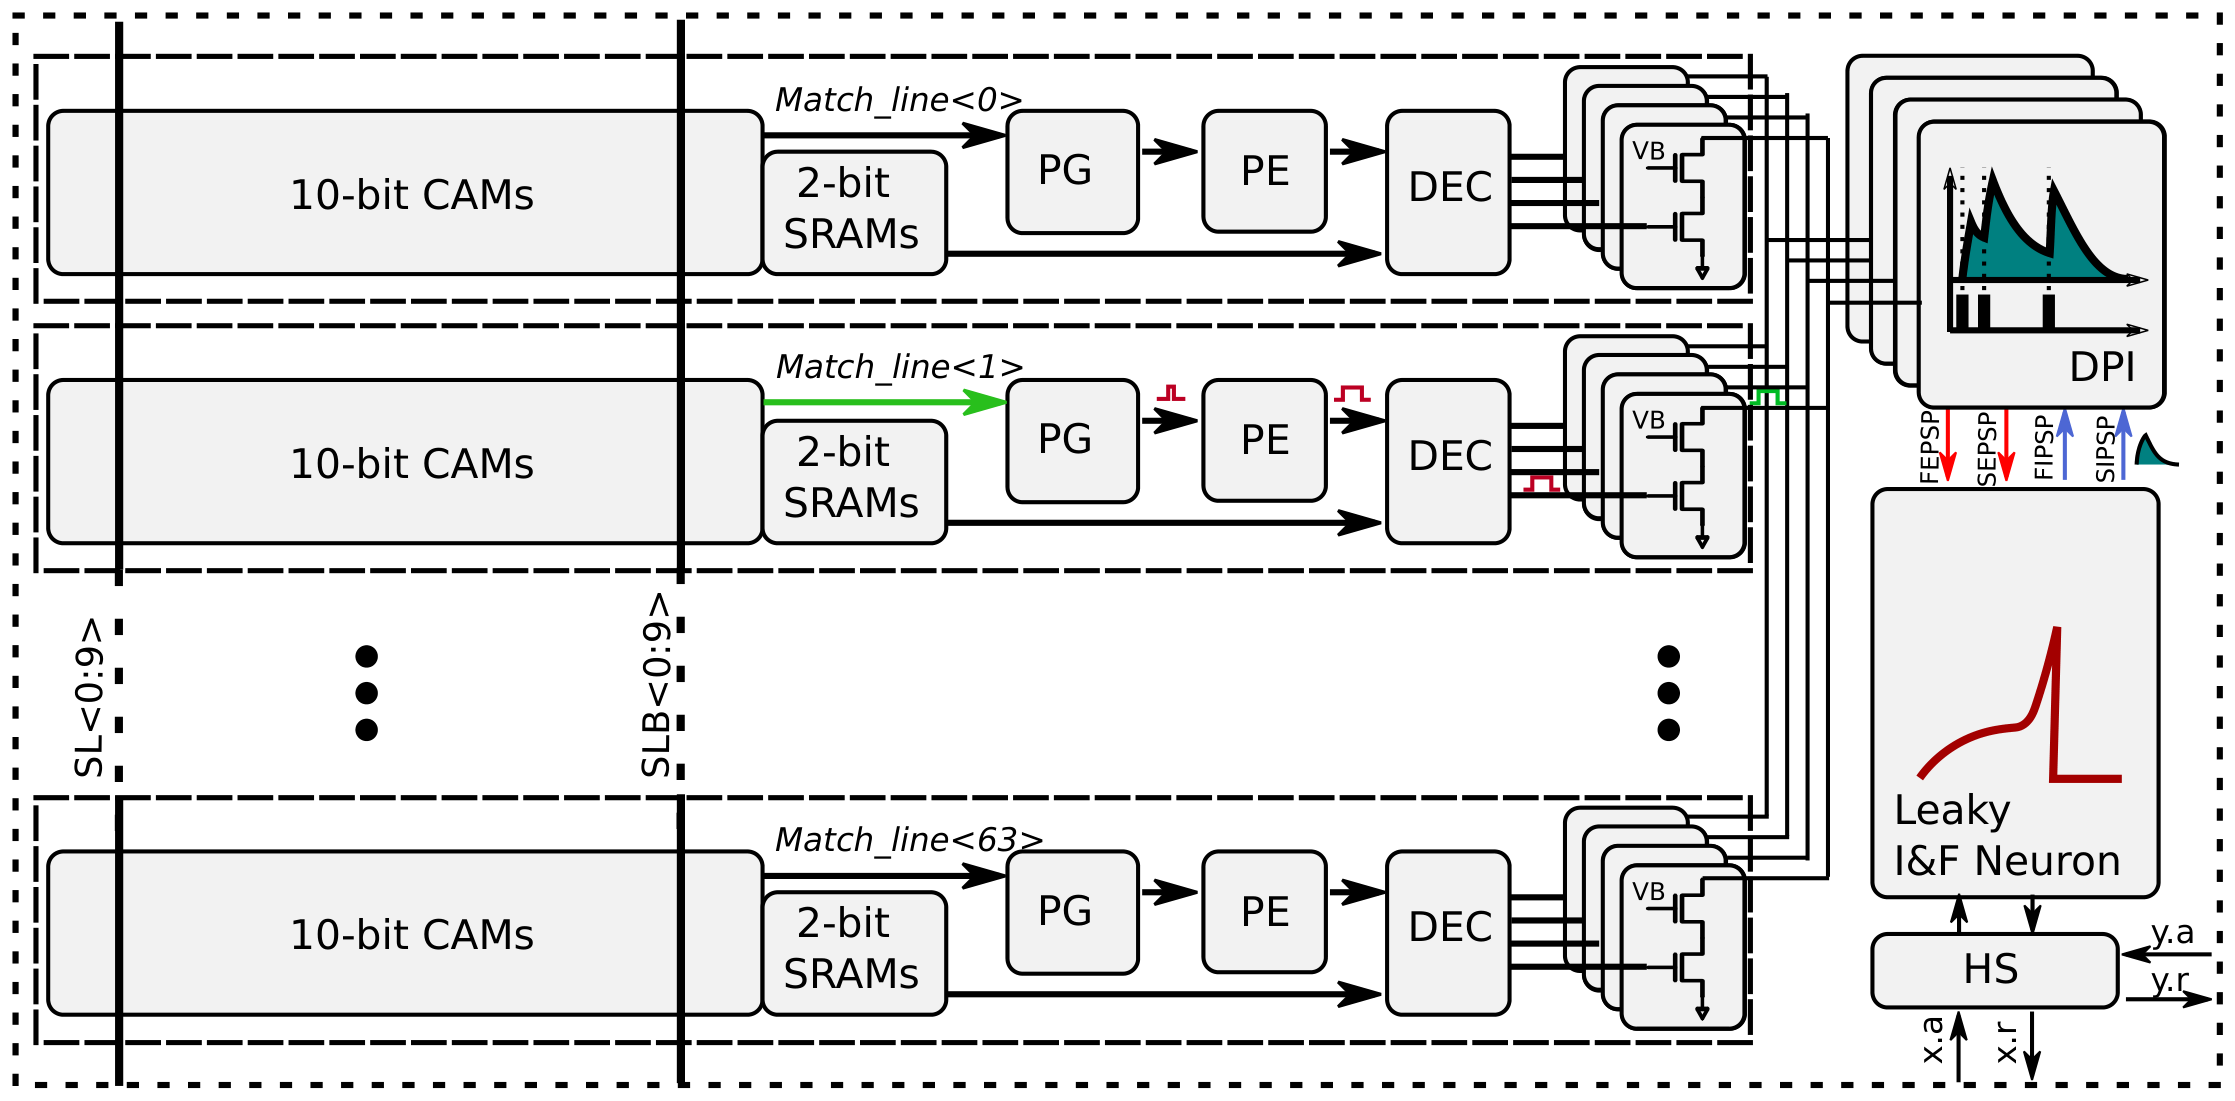
\includegraphics[width=\linewidth]{dynaps_node.png}
    \caption{Schema a blocchi di uno dei 256 nodi \emph{in-memory} di ciascun core.}
  \end{subfigure}
  \caption[Architettura di routing e nodo \emph{in-memory} di DYNAPs]{Architettura del processore multi-core DYNAPs~\cite{moradi2018}: (a) rete di routing asincrona QDI gerarchica (router locali R1 per core, R2 ad albero multi-livello intra-chip e R3 a mesh 2D XY tra chip); (b) struttura del singolo nodo di calcolo e memoria eterogenea distribuita (64 CAM da 10 bit, 64 SRAM da 2 bit, generatori/estensori/decodificatori d'impulsi PG/PE/DEC, 4 filtri DPI e 1 neurone analogico Leaky I\&F con blocco di handshaking HS). Riprodotto da Moradi et al.\ (2018)~\cite{moradi2018}.}
  \label{fig:dynaps_routing}
\end{figure}

Il chip prototipo DYNAPs è fabbricato in CMOS \SI{180}{\nano\meter} 1P6M (\SI{43{,}79}{\milli\meter\squared} totali, \SI{38{,}5}{\milli\meter\squared} di core) con tensione di alimentazione riducibile fino a \SI{1{,}3}{\volt} (nominale \SI{1{,}8}{\volt}), e integra \textbf{4 core da 256 neuroni} (1024 neuroni AdEx-I\&F DPI, 64k sinapsi con fan-in 64 e fan-out 4k, 64k celle CAM + 4k SRAM). I router R1, R2 e R3 (Figura~\ref{fig:dynaps_routing}a) sono sintetizzati con logica digitale asincrona \emph{Quasi Delay-Insensitive} (QDI) a codifica \emph{dual-rail} (latenza di attraversamento inter-chip di \SI{15{,}4}{\nano\second}, latenza interna di R3 di \SI{2{,}5}{\nano\second}, energia per \emph{hop} di \SI{17}{\pico\joule} a \SI{1{,}3}{\volt}, tempo di broadcast nella CAM di \SI{27}{\nano\second})~\cite{moradi2018}. Come visibile nella Figura~\ref{fig:dynaps_silicio}a (ingrandimento del nodo) e nella Tabella~I di Moradi et al.~\cite{moradi2018}, la memoria on-chip (31,7\%), gli estensori/decodificatori d'impulsi (25,2\%) e i router (9,7\%) occupano complessivamente il \textbf{66,6\%} dell'area core, mentre neuroni e sinapsi analogiche rappresentano solo il \textbf{22,8\%}. Ancora più illuminante è la Figura~\ref{fig:dynaps_silicio}b: al crescere della frequenza di firing fino a \SI{100}{\hertz}, la potenza della logica digitale di routing e CAM cresce molto più rapidamente di quella analogica, arrivando a rappresentare circa i due terzi della dissipazione totale a \SI{1{,}8}{\volt} ($\sim\SI{1{,}8}{\milli\watt}$ digitali su $\sim\SI{2{,}7}{\milli\watt}$ totali)~\cite{moradi2018}.

\begin{figure}[tb]
  \centering
  \begin{subfigure}[b]{0.52\textwidth}
    \centering
    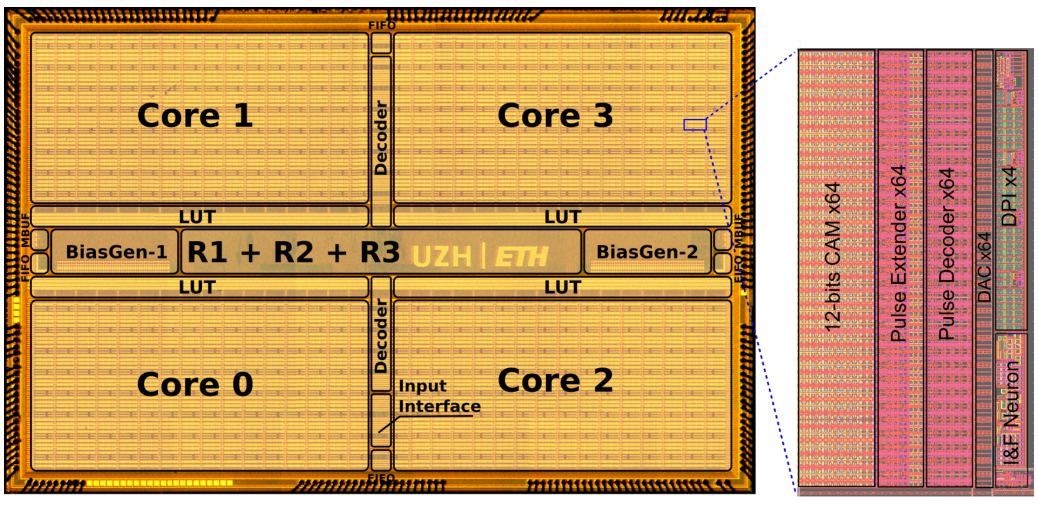
\includegraphics[width=\linewidth]{dynaps_die.png}
    \caption{Microfotografia del die DYNAPs (\SI{43{,}79}{\milli\meter\squared}) e zoom del nodo.}
  \end{subfigure}
  \hfill
  \begin{subfigure}[b]{0.45\textwidth}
    \centering
    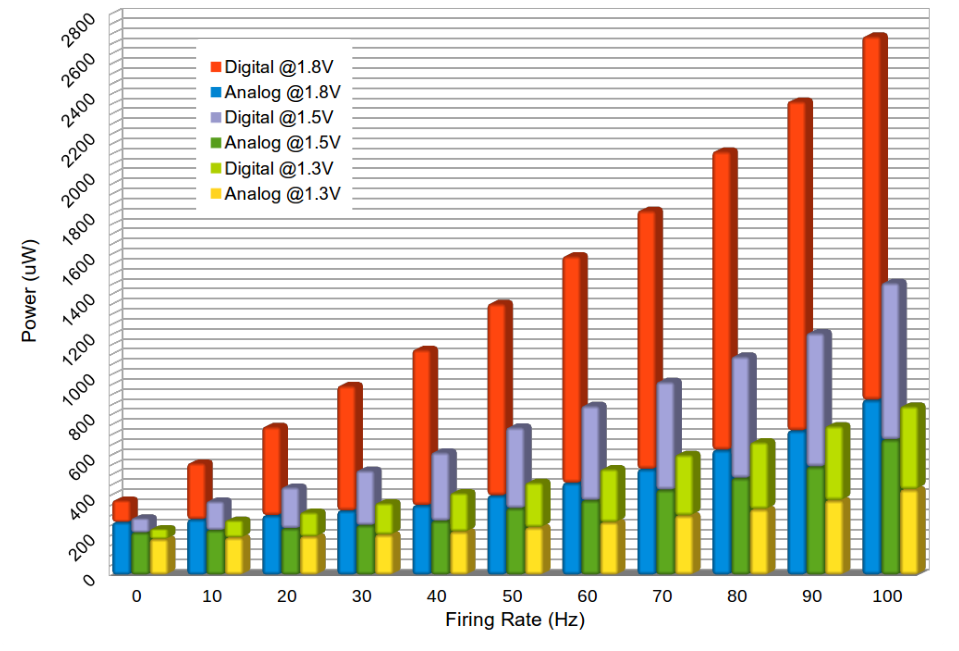
\includegraphics[width=\linewidth]{dynaps_power_freq.png}
    \caption{Potenza analogica e digitale misurata vs frequenza di firing.}
  \end{subfigure}
  \caption[Caratterizzazione hardware del processore DYNAPs]{Caratterizzazione hardware del processore multi-core DYNAPs~\cite{moradi2018}: (a) layout dei 4 core, router R1/R2/R3 e BiasGen, con dettaglio del singolo nodo che evidenzia l'ampia superficie occupata da CAM e Pulse Extender/Decoder rispetto al piccolo neurone I\&F e ai 4 DPI; (b) potenza totale impilata (analogica in basso, digitale in alto) al variare della frequenza di disparo di tutti i 1024 neuroni per $\Vdd = 1{,}3; 1{,}5; \SI{1{,}8}{\volt}$. Riprodotto da Moradi et al.\ (2018)~\cite{moradi2018}.}
  \label{fig:dynaps_silicio}
\end{figure}

L'evoluzione successiva \textbf{DYNAP-SE2} (utilizzata da Bartels et al.~\cite{bartels2025}) mantiene la medesima architettura \emph{mixed-signal} a 4 core in \SI{180}{\nano\meter} con neuroni AdEx-I\&F DPI e sinapsi a 4 tipi (AMPA, NMDA, GABA-A shunting, GABA-B), aggiungendo però l'AFE+ADM sullo stesso die e pesi a 4 bit; il suo \emph{mismatch} misurato sui parametri di bias sottosoglia ha un coefficiente di variazione (CV) del \textbf{20--30\%}, che gli autori compensano sfruttando la topologia ricorrente/NLNG anziché pesi precisi~\cite{bartels2025}. Per contrasto, il chip \textbf{Xylo} (Li et al.~\cite{li2024}) rappresenta il polo \textbf{interamente digitale} (CMOS \SI{28}{\nano\meter}, \SI{6{,}5}{\milli\meter\squared}, $\Vdd = \SI{1{,}8}{\volt}$ core / \SI{2{,}5}{\volt} I/O, clock fino a \SI{250}{\mega\hertz}, \SI{124}{\kilo\byte} SRAM): i 1000 neuroni LIF digitali con decadimento \emph{bit-shift} e pesi a 8 bit presentano \textbf{zero \emph{mismatch} analogico} e pieno supporto al training off-chip tramite BPTT, ma al prezzo di un consumo stabile di \SI{287{,}9}{\micro\watt} nel core (più \SI{87{,}4}{\micro\watt} I/O) e di una piccola perdita di accuratezza dovuta alla quantizzazione ($\sim 3{,}4\text{--}4{,}3$ punti percentuali)~\cite{li2024}.

\subsection{Tabelle comparative e risposta alla seconda domanda centrale}
\label{subsec:tabelle_cmos}

Le Tabelle~\ref{tab:confronto_neuroni} e~\ref{tab:confronto_sistemi} (riportate in formato orizzontale nelle pagine seguenti per la massima leggibilità) raccolgono sistematicamente tutti i parametri richiesti dalla consegna (tensione di alimentazione, consumo statico, potenza media, energia per spike, area, frequenza di firing e variabilità) rispettivamente a livello di singolo neurone CMOS e a livello di processore/sistema integrato. I campi non riportati esplicitamente dagli articoli originali sono indicati con ``\ND''.

\begin{sintesiBox}{Risposta alla Domanda Centrale 2: Come si realizza un neurone spiking in CMOS e quali compromessi emergono?}
Un neurone spiking CMOS integra quattro funzioni fisiche: accumulo di carica con perdita su una capacità di membrana ($\Cmem$), innesco rapido al superamento della soglia (tramite amplificatore/comparatore o feedback positivo in corrente), ripristino con periodo refrattario ($C_R$ / \emph{starved inverters}) ed eventualmente una seconda variabile lenta di adattamento (DPI di AHP o condensatore $C_u$). Le architetture proposte evidenziano un compromesso netto tra quattro assi:
\begin{itemize}
  \item \textbf{Analogico sottosoglia puro (DPI, Izhikevich a \SI{250}{\milli\volt}):} minimizza tensione, potenza (pW--nW) e area con costanti di tempo biologiche naturali \emph{real-time}, ma soffre di \textbf{elevata variabilità (\emph{mismatch} 9--30\%)} e ridotta capacità di pilotaggio, richiedendo sovradimensionamento selettivo (ROLLS), reti tolleranti alla topologia (DYNAP-SE2) o apprendimento/calibrazione.
  \item \textbf{Mixed-signal (neuroni analogici + routing/memorie digitali asincrone):} consente reti scalabili, programmabili e multi-core (ROLLS, DYNAPs, DYNAP-SE2), ma sposta gran parte di area ed energia dalle celle neuronali alle sinapsi, alle CAM e al routing AER.
  \item \textbf{Soprasoglia accelerato e Switched-Capacitor:} abbatte drasticamente il \emph{mismatch} e offre alta ripetibilità (10 regimi in Mihalas--Niebur S-C; $<10\text{ pJ/spike}$ in Izhikevich accelerato), ma perde la corrispondenza diretta col tempo reale biologico oppure introduce la distribuzione di clock multifase.
  \item \textbf{Completamente digitale (Xylo, I\&F full-custom):} elimina ogni variabilità analogica e facilita il training con algoritmi standard (BPTT), ma richiede SRAM dedicata, quantizzazione dei pesi e un consumo statico/dinamico dell'ordine di centinaia di microwatt.
\end{itemize}
\end{sintesiBox}

\begin{landscape}
\begin{table}[p]
  \centering
  \caption[Confronto tra implementazioni CMOS di singoli neuroni spiking]{Confronto tra le principali implementazioni CMOS di \textbf{singoli neuroni spiking} analizzate nella bibliografia~\cite{indiveri2011, qiao2015, ronchini2023}.}
  \label{tab:confronto_neuroni}
  \footnotesize
  \setlength{\tabcolsep}{4pt}
  \begin{tabularx}{\linewidth}{@{}L{2.85cm} L{3.35cm} L{1.55cm} L{1.2cm} L{3.0cm} L{3.0cm} L{2.85cm} Y@{}}
    \toprule
    \textbf{Neurone CMOS} & \textbf{Stile / Modello} & \textbf{Tecn.} & \textbf{$\Vdd$} & \textbf{Pot.\ / En.\ per spike} & \textbf{Area neurone} & \textbf{Scala temp.\ / Firing} & \textbf{Variabilità / Mismatch} \\
    \midrule
    \textbf{Axon-Hillock}~\cite{indiveri2011} & Sub-$V_T$, V-mode, I\&F base & CMOS std & \ND & Alta (cortocircuito inverter) & Molto compatta & \emph{Real-time} & Basso (dominato da $C_{\mathrm{fb}}/\Cmem$) \\
    \textbf{van Schaik OTA}~\cite{indiveri2011} & Sub-$V_T$, V-mode, I\&F + refr. & CMOS std & \ND & Ridotta vs Axon-H. & Compatta & \emph{Real-time} & Soglia esplicita $\Vthr$; mismatch OTA \\
    \textbf{Octopus Retina}~\cite{indiveri2011} & Sub-$V_T$, I\&F + fb corrente & \SI{0{,}6}{\micro\meter} & \ND & \textbf{$<\SI{4}{\pico\joule\per\spike}$} & Compatta (pixel) & \emph{Real-time} (spike ns) & Mismatch di soglia inverter \\
    \textbf{DVS ON/OFF}~\cite{indiveri2011} & Sub-$V_T$, diff.\ capacitivo & \SI{0{,}35}{\micro\meter} & \ND & Ultra-bassa & Compatta (pixel) & \emph{Real-time} ($f_c \approx \SI{0{,}05}{\hertz}$) & \textbf{Molto basso:} $\sim 2\%$ ($1\sigma$, \SI{1}{\milli\volt} eff.) \\
    \textbf{LLN (LPF)}~\cite{indiveri2011} & Sub-$V_T$, I-mode, cubico 2D & \SI{0{,}25}{\micro\meter} & \ND & $50\text{--}\SI{1000}{\nano\watt}$ & Compatta (16 MOS) & \emph{Real-time} ($\tau_g\sim\SI{100}{\milli\second}$) & Elevato (sottosoglia non calibrato) \\
    \textbf{DPI (ROLLS)}~\cite{indiveri2011, qiao2015} & Sub-$V_T$, I-mode, AdEx-I\&F & \SI{180}{\nano\meter} & \ND\textsuperscript{a} & Pochi \SI{}{\pico\joule\per\spike}\textsuperscript{b} & \SI{917{,}8}{\micro\meter\squared} ($55{,}7\times\SI{16{,}5}{\micro\meter}$) & \emph{Real-time} ($0\text{--}\SI{140}{\hertz}$ mis.) & \textbf{9,4\%} medio su curva $f\text{--}I$ (transistori larghi) \\
    \textbf{NET-TEN}~\cite{ronchini2023} & Sub-$V_T$, V-mode, Izhikevich & \SI{180}{\nano\meter} & \SI{0{,}25}{\volt} & $\sim\SI{0{,}12}{\nano\watt}$/n.\ med.\textsuperscript{c} & \SI{1476{,}84}{\micro\meter\squared} & \emph{Real-time} (ISI $\sim 4\text{--}\SI{8}{\milli\second}$) & Elevato (solo 4/10 canali utili senza taratura per cella) \\
    \textbf{Quadratic I\&F}~\cite{indiveri2011} & Soprasoglia, V-mode, Izhik. & \SI{0{,}35}{\micro\meter} & \ND & \textbf{$<\SI{10}{\pico\joule\per\spike}$} & Compatta (14 MOS) & Accelerato ($10^4\times$) & Basso (inversione forte) \\
    \textbf{S-C Mihalas--N.}~\cite{indiveri2011} & Switched-Cap, soglia adatt. & CMOS std & \ND & Media (clock multif.) & Media (modulare) & \emph{Real-time} (clockato) & \textbf{Molto basso} (rapporti capacitivi) \\
    \textbf{Charge-Packet}~\cite{indiveri2011} & Mixed, specchi calibrati & \SI{0{,}35}{\micro\meter} & \ND & Bassa (spike \SI{100}{\nano\second}) & \SI{8100}{\micro\meter\squared} ($90\times\SI{90}{\micro\meter}$) & \emph{Real-time} / veloce & Calibrato a 5 bit con Digi-MOS (3 bit+segno) \\
    \textbf{Digitale I\&F}~\cite{indiveri2011} & Full-custom digitale & \SI{0{,}35}{\micro\meter} & \ND & Dinamica da clock/agg. & \SI{10000}{\micro\meter\squared} ($100\times\SI{100}{\micro\meter}$) & Alta (spike \SI{50}{\nano\second}) & \textbf{Nullo} (18 bit accum., 5 bit+s pesi) \\
    \bottomrule
    \multicolumn{8}{@{}p{\linewidth}@{}}{\scriptsize \textsuperscript{a} Non esplicitata in~\cite{qiao2015} (processo \SI{180}{\nano\meter}; in Fig.~4 di~\cite{qiao2015} $\Vmem$ raggiunge $\sim\SI{1{,}3}{\volt}$). \textsuperscript{b} Stima per il nucleo DPI puro da~\cite{indiveri2011}; in DYNAPs~\cite{moradi2018} l'energia comprensiva di stadio AER/core sale a \SI{260}{\pico\joule} (\SI{1{,}3}{\volt}) o \SI{883}{\pico\joule} (\SI{1{,}8}{\volt}). \textsuperscript{c} Media indicativa su 30 neuroni + 30 sinapsi (\SI{3{,}50}{\nano\watt} totali; statico \SI{0{,}68}{\pico\watt} totali).}
  \end{tabularx}
\end{table}

\begin{table}[p]
  \centering
  \caption[Confronto tra processori e sistemi neuromorfici integrati]{Confronto a livello di \textbf{processori e sistemi neuromorfici integrati} della bibliografia~\cite{qiao2015, ronchini2023, moradi2018, bartels2025, li2024, wu2026}.}
  \label{tab:confronto_sistemi}
  \footnotesize
  \setlength{\tabcolsep}{4pt}
  \begin{tabularx}{\linewidth}{@{}L{2.65cm} L{3.25cm} L{1.85cm} L{2.25cm} L{2.95cm} L{3.25cm} L{3.05cm} Y@{}}
    \toprule
    \textbf{Sistema} & \textbf{Tecn.\ / Architettura} & \textbf{$\Vdd$} & \textbf{Pot.\ statica} & \textbf{Pot.\ media / dinamica} & \textbf{Energia per spike / evento} & \textbf{Area chip (neuroni \%)} & \textbf{Firing / Variabilità} \\
    \midrule
    \textbf{ROLLS}~\cite{qiao2015} & \SI{180}{\nano\meter} Mixed-sig.\ (256n, 128k sin.) & \ND\textsuperscript{a} & \ND & $\sim\SI{4}{\milli\watt}$ (attrattori) & \ND & \SI{51{,}4}{\milli\meter\squared} (neur.\ \textbf{0,47\%}, sin.\ 64,7\%) & $5\text{--}\SI{140}{\hertz}$; mismatch $f\text{--}I$ \textbf{9,4\%} \\
    \textbf{NET-TEN}~\cite{ronchini2023} & \SI{180}{\nano\meter} Analog.\ sub-$V_T$ (30n, 30 sin.) & \SI{0{,}25}{\volt} (\SI{0{,}3}{\volt} cont.) & \textbf{\SI{0{,}68}{\pico\watt}} & \textbf{\SI{3{,}50}{\nano\watt}} (+ \SI{31}{\pico\watt} cont.) & Cont.\ \SI{11{,}4}{\femto\joule\per\spike} (\SI{148{,}2}{\femto\joule\per\class}) & \SI{1{,}08}{\milli\meter\squared} (1n = \SI{1477}{\micro\meter\squared}) & \emph{Real-time} LFP; mismatch alto (4/10 ch utili) \\
    \textbf{DYNAPs}~\cite{moradi2018} & \SI{180}{\nano\meter} Multi-core (1k n, 64k sin.) & \SI{1{,}3}{\volt}--\SI{1{,}8}{\volt} & $\sim 250\text{--}\SI{390}{\micro\watt}$\textsuperscript{b} & $0{,}87\text{--}\SI{2{,}7}{\milli\watt}$ (1k n @ \SI{100}{\hertz}) & Gen.\ \SI{260}{\pico\joule}; CAM bcast \textbf{\SI{2{,}2}{\nano\joule}} (@ \SI{1{,}3}{\volt}) & \SI{43{,}79}{\milli\meter\squared} (core \SI{38{,}5}{\milli\meter\squared}; n+s 22,8\%) & $0\text{--}\SI{100}{\hertz}$ (38 Meps/core); mismatch sub-$V_T$ \\
    \textbf{DYNAP-SE2}~\cite{bartels2025} & \SI{180}{\nano\meter} Mixed-sig.\ + AFE/ADM (1k n) & \SI{1{,}8}{\volt} & \ND & \SI{150}{\micro\watt} (\SI{2{,}8}{\micro\watt\per\ch}) & Modello DYNAPs (\SI{883}{\pico\joule} gen., \SI{6{,}84}{\nano\joule} bcast) & 4 core + AFE (processo \SI{180}{\nano\meter}) & $10\text{--}\SI{600}{\hertz}$; CV bias \textbf{20--30\%} \\
    \textbf{Xylo}~\cite{li2024} & \SI{28}{\nano\meter} Digitale (1k LIF, 124 KB SRAM) & \SI{1{,}8}{\volt} core / \SI{2{,}5}{\volt} I/O & Inclusa nei \SI{288}{\micro\watt} & \SI{287{,}9}{\micro\watt} core + \SI{87{,}4}{\micro\watt} I/O & \ND & \SI{6{,}5}{\milli\meter\squared} & Clock \SI{250}{\mega\hertz}; mismatch \textbf{0\%} (quant.\ 8 bit) \\
    \textbf{NeuroSEED}~\cite{wu2026} & \SI{40}{\nano\meter} SoC 32 ch (AFE + ASC + Det. + UWB) & \SI{1{,}2}{\volt} / \SI{0{,}6}{\volt} & Ridotta (\emph{power-gating}) & \textbf{\SI{63{,}61}{\micro\watt}} tot.\ (\SI{1{,}38}{\micro\watt\per\ch} rec.) & UWB \SI{17{,}16}{\pico\joule\per\bit} (\SI{0{,}78}{\nano\joule}/tx-bit eff.) & \SI{0{,}70}{\milli\meter\squared} die (\SI{0{,}16}{\milli\meter\squared} att.; \SI{0{,}0032}{\milli\meter\squared}/ch AFE) & AP biologici ($f_s=\SI{10{,}4}{\kilo\hertz}$/ch); servo EDO $\pm\SI{50}{\milli\volt}$ \\
    \bottomrule
    \multicolumn{8}{@{}p{\linewidth}@{}}{\scriptsize \textsuperscript{a} Non dichiarata esplicitamente in~\cite{qiao2015} (processo \SI{180}{\nano\meter}, nominale \SI{1{,}8}{\volt}). \textsuperscript{b} Letto dalla Fig.~11 di~\cite{moradi2018} a \SI{0}{\hertz} (da $\sim\SI{250}{\micro\watt}$ a \SI{1{,}3}{\volt} fino a $\sim\SI{390}{\micro\watt}$ a \SI{1{,}8}{\volt}).}
  \end{tabularx}
\end{table}
\end{landscape}
